\documentclass[a4paper]{article}


% import packages
\usepackage{graphicx}  % for \includegraphics with jpg,png,...
\usepackage[english,ngerman]{isodate, babel}  % ngerman: Neue Rechtschreibung
\usepackage{url}
\usepackage[T1]{fontenc}
\usepackage[utf8]{inputenc}
\usepackage{textcomp}  % support for symbols like €
\usepackage{lmodern}  % improve font
\usepackage{float}  % allow H option in \begin{subfigure}[H]
\usepackage{caption}
\usepackage{hyperref}
\usepackage{subcaption}
\usepackage[%
backend=biber,
sorting=none,
natbib=true,
style=numeric,
autocite=inline
]{biblatex}
\addbibresource{references.bib}


% configure packages
\setlength{\columnsep}{8mm}
\setlength{\parindent}{7ex}

% redefine hyperref names
\addto\extrasngerman{
	\renewcommand{\sectionautorefname}{Kapitel}
	\renewcommand{\subsectionautorefname}{Abschnitt}
	\renewcommand{\subsubsectionautorefname}{Abschnitt}
}

\setlength{\parindent}{0cm}  % remove paragraph indentation
\setlength{\intextsep}{8pt}  % set space between two float objects

\raggedbottom  % move spacing produced by figures to the bottom of the page


\begin{document}

\title{\textbf{Dokumentation\\der Android-Anwendung\\"`stock simulator"'}}

\author{
    Jan Müller\\
    Jonas Thelemann\\
    Juri Lozowoj\\
    Lucas Held
}
\maketitle

\begin{figure}[H]
    \centering
    
\includegraphics[width=\textwidth,keepaspectratio]{./images/stock-simulator-social.png}
\end{figure}

\pagebreak
\tableofcontents
\pagebreak


\section{Einleitung}
\label{sec:introduction}
% Gute Einleitung ins Thema (was war die Aufgabe, etc.)
Im Rahmen der Blockveranstaltung \textit{Code-Camp Context-Awareness 1} des Fachgebiets \textit{Kommunikationstechnik} im Fachbereich \textit{16 - Elektrotechnik/Informatik} der Universität Kassel entwickelten mehrere Teams von drei bis vier Studenten innerhalb einer Woche selbstständig ein Börsensimulationsspiel für Android-Smartphones. Dabei stellt die Verwendung von \textbf{echten, aktuellen Anlagekursen} eine wichtige Anforderung an das Spiel dar. Mithilfe von zur Verfügung stehendem \textbf{Spielgeld} soll der Benutzer die Möglichkeit haben, mit Anlagen, wie Aktien oder Kryptowährungen, zu handeln. Um den Handel mit verschiedenen Anlagen zu ermöglichen, wird eine \textbf{Suchfunktion} gefordert, welche die verfügbaren Anlagen filtert und anzeigt. Um das eigene Budget immer im Blick zu behalten, sollen eine \textbf{Depotübersicht} sowie eine Anzeige für den aktuellen \textbf{Kontostand} und dessen Verlauf erstellt werden. Die getätigten Käufe und Verkäufe sollen in einer \textbf{Historie} bzw. einem Transaktionsverlauf dargestellt werden. \textbf{Graphen} sollen die Anlagenkurse und den Verlauf des Kontostands visualisieren. Wie auf gängigen Handelsplattformen üblich, soll der Simulator auch mit jedem Kauf- oder Verkauf \textbf{Transaktionskosten} erheben. Das Handeln soll optional durch einen \textbf{Bot} automatisiert werden können. Entsprechende Zielwerte für den automatisierten Handel sollen für jede Anlage individuell anpassbar sein. Damit der Benutzer die Möglichkeit hat, das Spiel neu zu beginnen, soll die Anwendung eine Option bieten, den \textbf{Spielstand zurückzusetzen}. Zusätzlich zu den bisher genannten Hauptfeatures, wird mindestens ein \textbf{Zusatzfeature} gefordert, welches eine nützliche Erweiterung für die Anwendung darstellt. Ziel des Spiels ist es, durch den erfolgreichen Handel mit Anlagemöglichkeiten das Startkapital zu vermehren.

Am 18.11.2019, drei Monate vor Beginn des Code-Camps selbst, fand die Vorbesprechung zur Veranstaltung statt. Neben allgemeinen Informationen zum Ablauf, wurden die Teilnehmer angewiesen, sich in die Software-Entwicklung für Android einzuarbeiten. Neben den dort vorgestellten Verweisen auf Lehrmaterial, arbeiteten sich die meisten Mitglieder unseres Teams mithilfe des Kurses \textit{Developing Android Apps with Kotlin} der Plattform \textit{Udacity}\footnote{Siehe \url{https://classroom.udacity.com/courses/ud9012}} in die App-Entwicklung für Android-Smartphones ein. Zu Beginn wird in diesem Kurs das Erstellen einer ersten, einfachen Android-App erklärt. Dann werden Konzepte wie Layouts, App-Navigation sowie der Activity- und Fragment-Lebenszyklus erläutert. Nach weiteren Kapiteln zur Benutzeroberfläche und Datenspeicherung, wird der \textit{RecyclerView} vorgestellt. Mit Retrofit wird beispielhaft das Beziehen von Daten aus Web-APIs umgesetzt. Nach einem Blick auf Android-Hintergrunddienste stellt der Kurs zuletzt Möglichkeiten zur Internationalisierung und barrierefreien Gestaltung vor.


\section{Technische Details}
\label{sec:technologies}
In diesem Abschnitt wird detaillierter auf die technischen Hintergründe der Anwendung "`stock simulator"' eingegangen. Die verwendete App-Architektur wird erklärt und die eingesetzten APIs und Bibliotheken werden vorgestellt.


\subsection{Architektur}
\label{subsec:technologies:architecture}
% App Architektur (Welches Pattern habt ihr benutzt? MVVM? Livedata?) Was ist das und warum ist das cool?
% Schwierigkeiten und wie ihr sie gelöst habt
Die App-Architektur folgt offiziellen Empfehlungen \autocite{google_recommendations} und basiert auf einer sog. \textit{Activity} sowie dem \textit{Model-View-ViewModel-Pattern} (MVVM).
Bei diesem Entwurfsmuster werden Präsentation der Benutzeroberfläche, Logik und Datenquellen voneinander getrennt (siehe \autoref{fig:technologies:architecture:mvvm}).
Benutzeroberflächen sind in dieser Anwendung durch \textit{Fragments} realisiert und ihre Logik in \textit{ViewModels} implementiert.
Benutzeroberflächenunabhängige Logik residiert in \textit{Repositories}.
Durch diese Trennung ist es möglich die MVVM-Schichten separat voneinander zu testen.
Das MVVM-Entwurfsmuster ermöglicht außerdem eine Wiederverwendung von \textit{ViewModels} und \textit{Models} in verschiedenen Fragmenten, da sie keine Informationen über spezifische UI-Elemente halten.

Die Navigation zwischen einzelnen \textit{Fragments} innerhalb der \textit{Activity} wird durch die \textit{Navigation} Libraries \autocite{android_navigation}, welche in Android Jetpack (siehe \autoref{subsubsec:technologies:bibs:jetpack}) enthaltenen sind, stark vereinfacht. Im Navigation Graph, einem graphischen Editor, werden zwischen den Elementen, den \textit{Fragments}, Verbindungen erstellt, um zu spezifizieren zwischen welchen \textit{Fragments} in welche Richtung navigiert werden kann.

Mithilfe von Lifecycle-Komponenten \autocite{android_lifecycle}, welche in Android Jetpack (siehe \autoref{subsubsec:technologies:bibs:jetpack}) enthalten sind, ist es möglich auf Statusänderungen anderer Life\-cycle-Komponenten zu reagieren. Dadurch wird strukturierterer und somit besser zu wartender Quellcode geschrieben. In dieser Anwendung wurde hauptsächlich von den Lifecycle-Komponenten \textit{LiveData}, \textit{MutableLiveData} und \textit{MediatorLiveData} Gebrauch gemacht.


\begin{figure}[H]
	\centering
	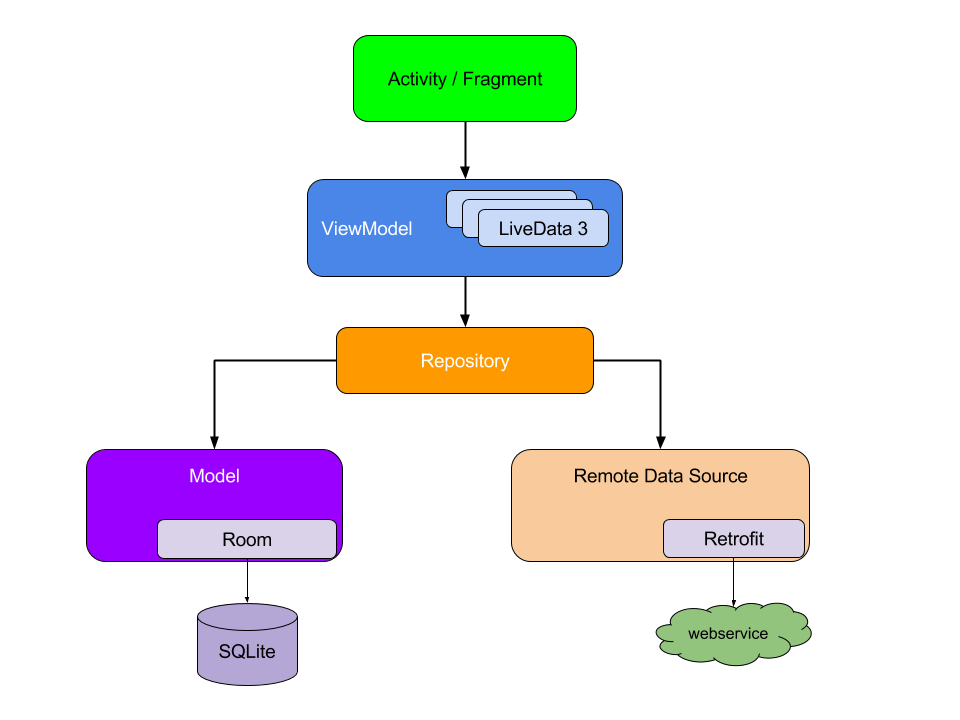
\includegraphics[height=8cm,keepaspectratio]{./images/mvvm-architecture.png}
	\caption{MVVM-Entwurfsmuster \autocite{mvvm_architecture}}
	\label{fig:technologies:architecture:mvvm}
\end{figure}

\textit{Fragmente} verwenden \textit{Databinding}, um von \textit{ViewModels} bereitgestellte Daten anzuzeigen.
Dabei handelt es sich um ein Feature des Compilers, welches benötigten Quelltext automatisch generiert, wodurch Fehleranfälligkeit reduziert und die Entwicklung beschleunigt wird.
Die Verwendung von \textit{LiveData} ermöglicht zudem eine automatische Aktualisierung von Benutzeroberflächen bei Veränderung des Datenbestandes.
\textit{LiveData} ist nicht nur ein generischer \textit{Wrapper}, sondern verfügt über einen automatisierten Lebenszyklus und kann sog. \textit{Observer} über Änderungen informieren.

In \textit{ViewModels} ist das Verhalten von Benutzeroberflächen definiert. Sie beziehen ihre Daten aus Datenquellen, welche in Form von \textit{Repositories} implementiert sind.
Einem \textit{ViewModel} ist das besitzende Fragment nicht bekannt, wodurch es unabhängig von Benutzeroberflächen verwendbar ist.

\textit{Repositories} dienen als \textit{Single Point of Truth}, wodurch fehlerhafte oder inkonsistente Datenbestände vermieden werden.
Sie sind an die interne Datenbank (siehe \autoref{subsubsec:technologies:bibs:room}) sowie verschiedene Netzwerkquellen (siehe \autoref{subsec:technologies:apis}) angebunden.


\subsection{APIs}
\label{subsec:technologies:apis}
Um eine Simulation mit echten Kursdaten zu ermöglichen, wurden zwei Applikationsschnittstellen als Datenquellen in "`stock simulator"' eingebunden.
Sie verwenden, trotz ähnlicher Semantik, unterschiedlich repräsentierte Datenstrukturen, weshalb auch in unserem Code separate Modelle für diese Datenstrukturen implementiert werden mussten.
Die API-spezifischen Antworten der Schnittstellen werden dann jedoch zu einem einheitlichen Datenmodell transformiert, so dass das Domänenmodell der App simpel und leichtgewichtig bleibt.
Beide APIs erfordern Zuschreibungen, welche im Settings-Screen eingesehen werden können (siehe \autoref{subsec:functionality:settings}).
Die nun folgenden individuellen API-Beschreibungen nennen nur von uns genutzte Endpunkte. Darüber hinaus bieten die APIs noch viele weitere Endpunkte.


\subsubsection{CoinGecko}
\label{subsubsec:technologies:apis:coingecko}
% https://www.coingecko.com/
\textit{CoinGecko}\footnote{Siehe \url{https://www.coingecko.com/}} stellt Informationen über Kryptowährungen bereit, die nicht kostenfrei über die IEX-Cloud API bezogen werden können (siehe \autoref{subsubsec:technologies:apis:iex}).
Dazu zählen Symbol, Name und Wechselkurse.
Bei Wechselkursen wird nur auf den USD-Wechselkurs zurückgegriffen.
Darüber hinaus sind Marktdiagrammdaten verfügbar, die für Kursgraphen verwendet werden.


\subsubsection{IEX Cloud}
\label{subsubsec:technologies:apis:iex}
% https://iexcloud.io/
\textit{IEX Cloud}\footnote{Siehe \url{https://iexcloud.io/}} stellt allgemeine Finanzdaten zur Verfügung.
Nicht alle Daten sind kostenlos zugänglich, weshalb nur Aktieninformationen über diese Schnittstelle bezogen werden.
Analog zu \textit{CoinGecko} (siehe \autoref{subsubsec:technologies:apis:coingecko}) liefert \textit{IEX Cloud} Symbole, Namen, aktuelle Preise und Marktdiagrammdaten zu Aktien.
Des Weiteren besitzt \textit{IEX Cloud} Informationen über kurzfristige Änderungen von Aktienkursen und bietet Sammlungen von Neuigkeiten zu einzelnen Aktien.


\subsection{Bibliotheken}
\label{subsec:technologies:bibs}
Im Laufe der Entwicklung wurden verschiedene Bibliotheken von Drittherstellern verwendet, um den notwendigen Programmierungsaufwand für unsere Anwendung zu reduzieren.
Im Folgenden werden die verwendeten Bibliotheken näher vorgestellt und ihre Vorzüge sowie Eigenschaften werden erläutert.


\subsubsection{Android Jetpack}
\label{subsubsec:technologies:bibs:jetpack}
Android Jetpack ist eine Sammlung von Bibliotheken, Programmen und Anleitungen. Ziel ist es, das Entwickeln von qualitativ hochwertigen Applikationen zu vereinfachen. Dies wird erreicht, indem dem Entwickler Komponenten vorgegeben werden, unter deren Verwendung weniger Boilerplate-Code geschrieben werden muss. Somit werden komplizierte Prozesse stark vereinfacht \autocite{android_jetpack}. Zu erkennen ist die Verwendung einer Jetpack Library in Code am Namespace \textit{androidx.*}. Die in Jetpack enthaltenen Libraries sind unabhängig von der Android Platform API verwendbar. Dadurch wird Abwärtskompatibilität zu älteren Android-Versionen gewährleistet und der Entwickler bekommt plattformunabhängige und häufigere Updates der Libraries. Die Android Jetpack Komponenten lassen sich in die vier Anwendungsgebiete \textit{Fundation}, \textit{Architecture}, \textit{Behavior} und \textit{UI} einteilen. \textit{Fundation} Komponenten stellen beispielweise die Abwärtskompatibilität sicher, beinhalten ein Testframework und ermöglichen das Arbeiten mit der Programmiersprache Kotlin. \textit{Architecture} Komponenten unterstützen den Programmierer, robusten, testbaren und wartbaren Quellcode zu schreiben. Beispielkomponenten für diesen Anwendungsbereich sind \textit{LiveData}, \textit{Data Binding}, \textit{Room} und der \textit{WorkManager}. \textit{Behavior} Komponenten ermöglichen den einfacheren Umgang mit Android Services, wie Benachrichtigungen, Kamera und Berechtigungen. \textit{UI} Komponenten erleichtern die Entwicklung der Benutzeroberfläche, beispielsweise durch \textit{Fragments}.

Zusätzlich zu den Libraries, welche in diesem Abschnitt erläutert werden, wurden weitere Libraries aus Android Jetpack verwendet, die im Folgenden vorgestellt werden.

\textit{Android KTX} erweitert die Sprache Kotlin um zusätzliche Funktionen, die hilfreich sind, um Kotlin unkompliziert in Kombination mit Android, Jetpack und anderen APIs nutzen zu können \autocite{android_ktx}.

\textit{Appcompat} \autocite{android_appcompat} ermöglicht die Nutzung der \textit{Action Bar} \autocite{android_action_bar} in der Benutzeroberfläche. Außerdem unterstützt diese Library das nachträgliche Hinzufügen vom \textit{material design} System, welches in \autoref{subsubsec:technologies:bibs:material} beschrieben ist.

\textit{Fragments} stellen ein Verhalten oder einen Teil der Benutzeroberfläche dar \autocite{android_fragments}. Eine \textit{Activity} ist modular aus mehreren \textit{Fragments} aufgebaut und ermöglicht es zur Laufzeit \textit{Fragments} hinzuzufügen oder zu entfernen.

\textit{Layouts} definieren die Anordnung der Benutzeroberfläche bzw. der \textit{Activities} \autocite{android_layouts}. Die Struktur wird hierarchisch aus allen Elementen aufgebaut, die dem Benutzer angezeigt werden sollen. Um die sichtbaren Elemente zu positionieren, können sogenannte, unsichtbare \textit{ViewGroup} Elemente zu Hilfe genommen werden. Verwendet wurden in dieser Applikation die \textit{ViewGroups} \textit{ConstraintLayout} \autocite{android_constraintlayout} und \textit{SwipeRefreshLayout} \autocite{android_swiperefreshlayout}. \textit{ConstraintLayouts} ermöglichen die Positionierung und Größenanpassung der Elemente in flexibler Weise. \textit{SwipeRefreshLayouts} werden immer dort verwendet, wo der Benutzer den Inhalt der Ansicht durch eine vertikale Wischgeste aktualisieren kann.


\subsubsection{Room}
\label{subsubsec:technologies:bibs:room}
% https://developer.android.com/jetpack/androidx/releases/room
Die Room-Persistenzbibliothek stellt eine Abstraktionsschicht über SQLite\footnote{Siehe \url{https://de.wikipedia.org/wiki/SQLite}} dar. Ihr Ziel ist es, Datenbankanfragen zu vereinfachen und "`die volle Leistung von SQLite zu nutzen"' \autocite{android_room_architecture}. Die Bibliothek hilft dabei, einen Cache der Anwendungsdaten auf dem Gerät zu erstellen. Dieser fungiert als Single Source of Truth und stellt sicher, dass eine konsistente Kopie der Anwendungsinformationen zur Verfügung steht. Durch die lokale Speicherung der Daten kann der Nutzer, auch offline, auf diese Inhalte zugreifen. Alle Inhaltsänderungen, die vom Benutzer vorgenommen werden, werden mit dem Server synchronisiert, sobald das Gerät wieder online ist.\newline
Room besteht im Wesentlichen aus drei Komponenten: \textit{Database}, \textit{Entity} und \textit{Dao}. \textit{Database} enthält den Datenbankinhaber und fungiert als Hauptzugriffspunkt für die Verbindung zu den persistenten Daten der Anwendung. \textit{Entity} entspricht einer Datenbanktabelle. \textit{Dao} beinhaltet die Methoden für den Zugriff auf die Datenbank. Die Anwendung nutzt die Room-Datenbank, um an die Data-Access-Objects (DAOs) zu gelangen. Anschließend werden die einzelnen DAOs verwendet, um die Entitäten aus der Datenbank abzurufen und Änderungen in die Datenbank zu schreiben. Die Entitäten werden dazu verwendet, um die entsprechenden Werte der Datenbanktabellen abzurufen und zu schreiben \autocite{android_room_data_storage}. Die Beziehung zwischen den drei Komponenten wird in Abbildung \ref{fig:room} dargestellt.

\begin{figure}[H]
	\centering
	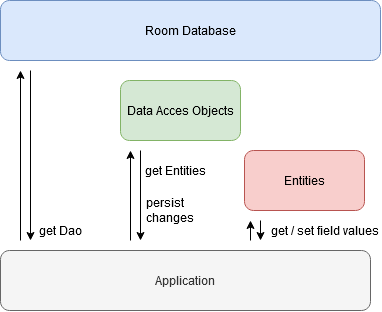
\includegraphics[height=7cm,keepaspectratio]{./images/Room.png}
	\caption{Room Architektur}
	\label{fig:room}
\end{figure}


\subsubsection{WorkManager}
\label{subsubsec:technologies:bibs:workmanager}
% https://developer.android.com/jetpack/androidx/releases/work
% https://developer.android.com/topic/libraries/architecture/workmanager
WorkManager ist eine in Android Jetpack enthaltene Bibliothek \autocite{android_workmanager}. Sie vereinfacht das Ausführen von Hintergrundaufgaben, sogenannten \textit{Workern}. Es existieren einmalige und periodische Worker. Mithilfe des WorkManagers werden die Worker besonders ressourcensparend, vor allem aber energiesparend, im Hintergrund ausgeführt. \textit{Constraints} ermöglichen es, Bedingungen an den Worker zu knüpfen, beispielweise das Benötigen einer Internetverbindung. Mittels \textit{Data} werden dem Worker Daten übergeben, welche gegebenenfalls für die Ausführung benötigt werden. Einmalige Worker eignen sich besonders für Aufgaben, die zurückgestellt werden können und nicht im Vordergrund zu erledigen sind. Periodische Worker können immer dort eingesetzt werden, wo mit den gleichen Einstellungen regelmäßig Arbeit verrichtet werden soll. Das kleinstmögliche Intervall ist bei periodischen Workern auf 15 Minuten beschränkt.


\subsubsection{Moshi}
\label{subsubsec:technologies:bibs:moshi}
% https://github.com/square/moshi
\textit{Moshi}, eine moderne JSON-Bibliothek für Kotlin und Java, erlaubt es ohne großen Aufwand, JSON zu Java-Objekten zu parsen und Java-Objekte zu JSON zu serialisieren \autocite{moshi}. Mit eingebauten Typadaptern können Javas Kerndatentypen, wie primitive Datentypen, Arrays, Strings und Enums, direkt von JSON gelesen und in JSON geschrieben werden. Über Annotationen können eigene Typadapter definiert werden. Moshi unterstützt die Kotlin Reflection Library\footnote{Siehe \url{https://kotlinlang.org/docs/reference/reflection.html}}, um Kotlin-Klassen von und zu JSON zu konvertieren.
In unserer Anwendung wird eine \textit{MoshiConverterFactory} von der Moshi-Instanz erzeugt und in Retrofit (siehe \autoref{subsubsec:technologies:bibs:retrofit}) verwendet.


\subsubsection{Retrofit}
\label{subsubsec:technologies:bibs:retrofit}
% https://github.com/square/retrofit
Mit \textit{Retrofit}, einem typsicheren HTTP-Client für Android und Java, können HTTP APIs in Java-Interfaces verwandelt werden \autocite{retrofit}. Unter Angabe einer Basis-URL wird eine Retrofit-Instanz für eine Klasse angelegt, in der sich annotierte Methoden befinden, anhand derer die API-Endpunkte definiert werden. Pfad-, Query-, Body- und Header-Parameter werden vollständig unterstützt. Mit dem Moshi-Converter\footnote{Siehe \texttt{com.squareup.retrofit2:converter-moshi}} können Server-Antworten direkt zu Java-Objekten deserialisiert werden (siehe \autoref{subsubsec:technologies:bibs:moshi}).


\subsubsection{MPAndroidChart}
\label{subsubsec:technologies:bibs:mpandroidchart}
% https://github.com/PhilJay/MPAndroidChart
\textit{MPAndroidChart} \autocite{mpandroidchart} ermöglicht die Darstellung von Diagrammen unter Android. Unterstützt werden alle gängigen Diagrammtypen sowie Kombinationen von mehreren Typen in einem Diagramm. Durch die vielen unterstützten Konfigurationsmöglichkeiten können die Diagramme passgenau auf das Anwendungsgebiet abgestimmt werden. In dieser Applikation wurden mithilfe der Bibliothek der Verlauf des Kontostands, des Depots und des Aktienkurses visualisiert.


\subsubsection{Biometric-Auth}
\label{subsubsec:technologies:bibs:biometricauth}
% https://github.com/anitaa1990/Biometric-Auth-Sample
Die Library \textit{Biometric-Auth} \autocite{biometricauth} vereinfacht die Implementierung einer Finger\-abdruck-Authentifizierung erheblich. Durch die Nutzung entfällt der normalerweise notwendige Boilerplate-Code für den Entwickler. Mithilfe dieser Library wurde die optionale Fingerabdruck-Authentifizierung implementiert, welche das Starten der Applikation ohne Authentifizierung verweigert (siehe \autoref{subsec:functionality:settings}).


\subsubsection{Picasso}
\label{subsubsec:technologies:bibs:picasso}
% https://github.com/square/picasso
\textit{Picasso} \autocite{picasso} ist eine Library, die das Herunterladen und Zwischenspeichern von Bildern ermöglicht. Durch die Zwischenspeicherung wird zum einen Datenvolumen gespart und zum anderen die Performance der Benutzeroberfläche bei mehrmaligen Aufrufen erhöht. In der Applikation wurde die Library für die Anzeige von News verwendet, welche mit Bildern ausgeliefert werden (siehe \autoref{subsec:functionality:news}).


\subsubsection{Material}
\label{subsubsec:technologies:bibs:material}
% https://material.io/develop/android/docs/getting-started/
\textit{Material} ist ein Designsystem, welches unter anderem von Google entwickelt wird.
Mit UI-Elementen der offiziellen \textit{Material}-Bibliothek ist es möglich, moderne Benutzeroberflächen zu erstellen ohne Entwicklungszeit für Design und Implementierung dieser aufwenden zu müssen.
\textit{Material} wurde für das App-Theme sowie die \textit{Bottom Navigation} (siehe \autoref{subsec:functionality:navigation}) verwendet.


\subsubsection{Timber}
\label{subsubsec:technologies:bibs:timber}
% https://github.com/JakeWharton/timber
\textit{Timber} ist eine Schnittstelle, welche auf der Android \textit{Log}-Klasse aufbaut und das Loggen von Ereignissen vereinfacht.
Durch Logging mit Timber ist es möglich, Entwicklungszeit zu sparen und Programmierfehler schnell ausfindig zu machen.
Log-Nachrichten werden von Timber nur während der Entwicklung und nicht in der fertigen App ausgegeben.


\subsubsection{Dokka}
\label{subsubsec:technologies:bibs:dokka}
% https://github.com/Kotlin/dokka
\textit{Dokka} ist eine "`documentation engine"' \autocite{dokka} und wird zum Generieren von Quelltextdokumentationen verwendet.
Es handelt sich also nicht um eine Bibliothek, die von der App verwendet wird, sondern um ein Entwicklungswerkzeug.
Mit \textit{Dokka}  wird die Dokumentation des Quelltextes dieser App generiert\footnote{Siehe \url{https://deryeger.github.io/stock-simulator/app/}}.


\section{Funktionalität}
\label{sec:functionality}
% Welche Features habt ihr gebaut?
% Welche Screens habt ihr gebaut?
% Warum sehen die Screens so aus? (warum ist button X an Position Y) / was habt ihr euch dabei gedacht?
Im Folgenden wird die Funktionalität der App, nach Screens aufgeteilt, vorgestellt.


\subsection{Navigation}
\label{subsec:functionality:navigation}
Über die \textit{Bottom Navigation} können Nutzer zwischen den Hauptfeatures Account, Suche, Transaktionsverlauf, Stockbrot und Errungenschaften wechseln.
Diese Art der Navigation wurde gewählt, da sie modernen Designempfehlungen \autocite{bottom_navigation} entspricht und bessere Kompatibilität mit Android 10 Gesten aufweist als beispielsweise ein \textit{Hamburger Menü}.

Das Einstellungsmenü ist über das Zahnrad in der Toolbar aller Screens, au"ser den Einstellungen selbst, erreichbar.

Weitere Navigation, wie zu den News oder zur Detailansicht einer Anlage, ist über Bedienelemente in Form von Buttons an entsprechenden Stellen möglich.

\autoref{fig:functionality:navigation:screens} stellt den Navigationsgraph zwischen den einzelnen Bildschirmen dar.
\begin{figure}[H]
	\centering
	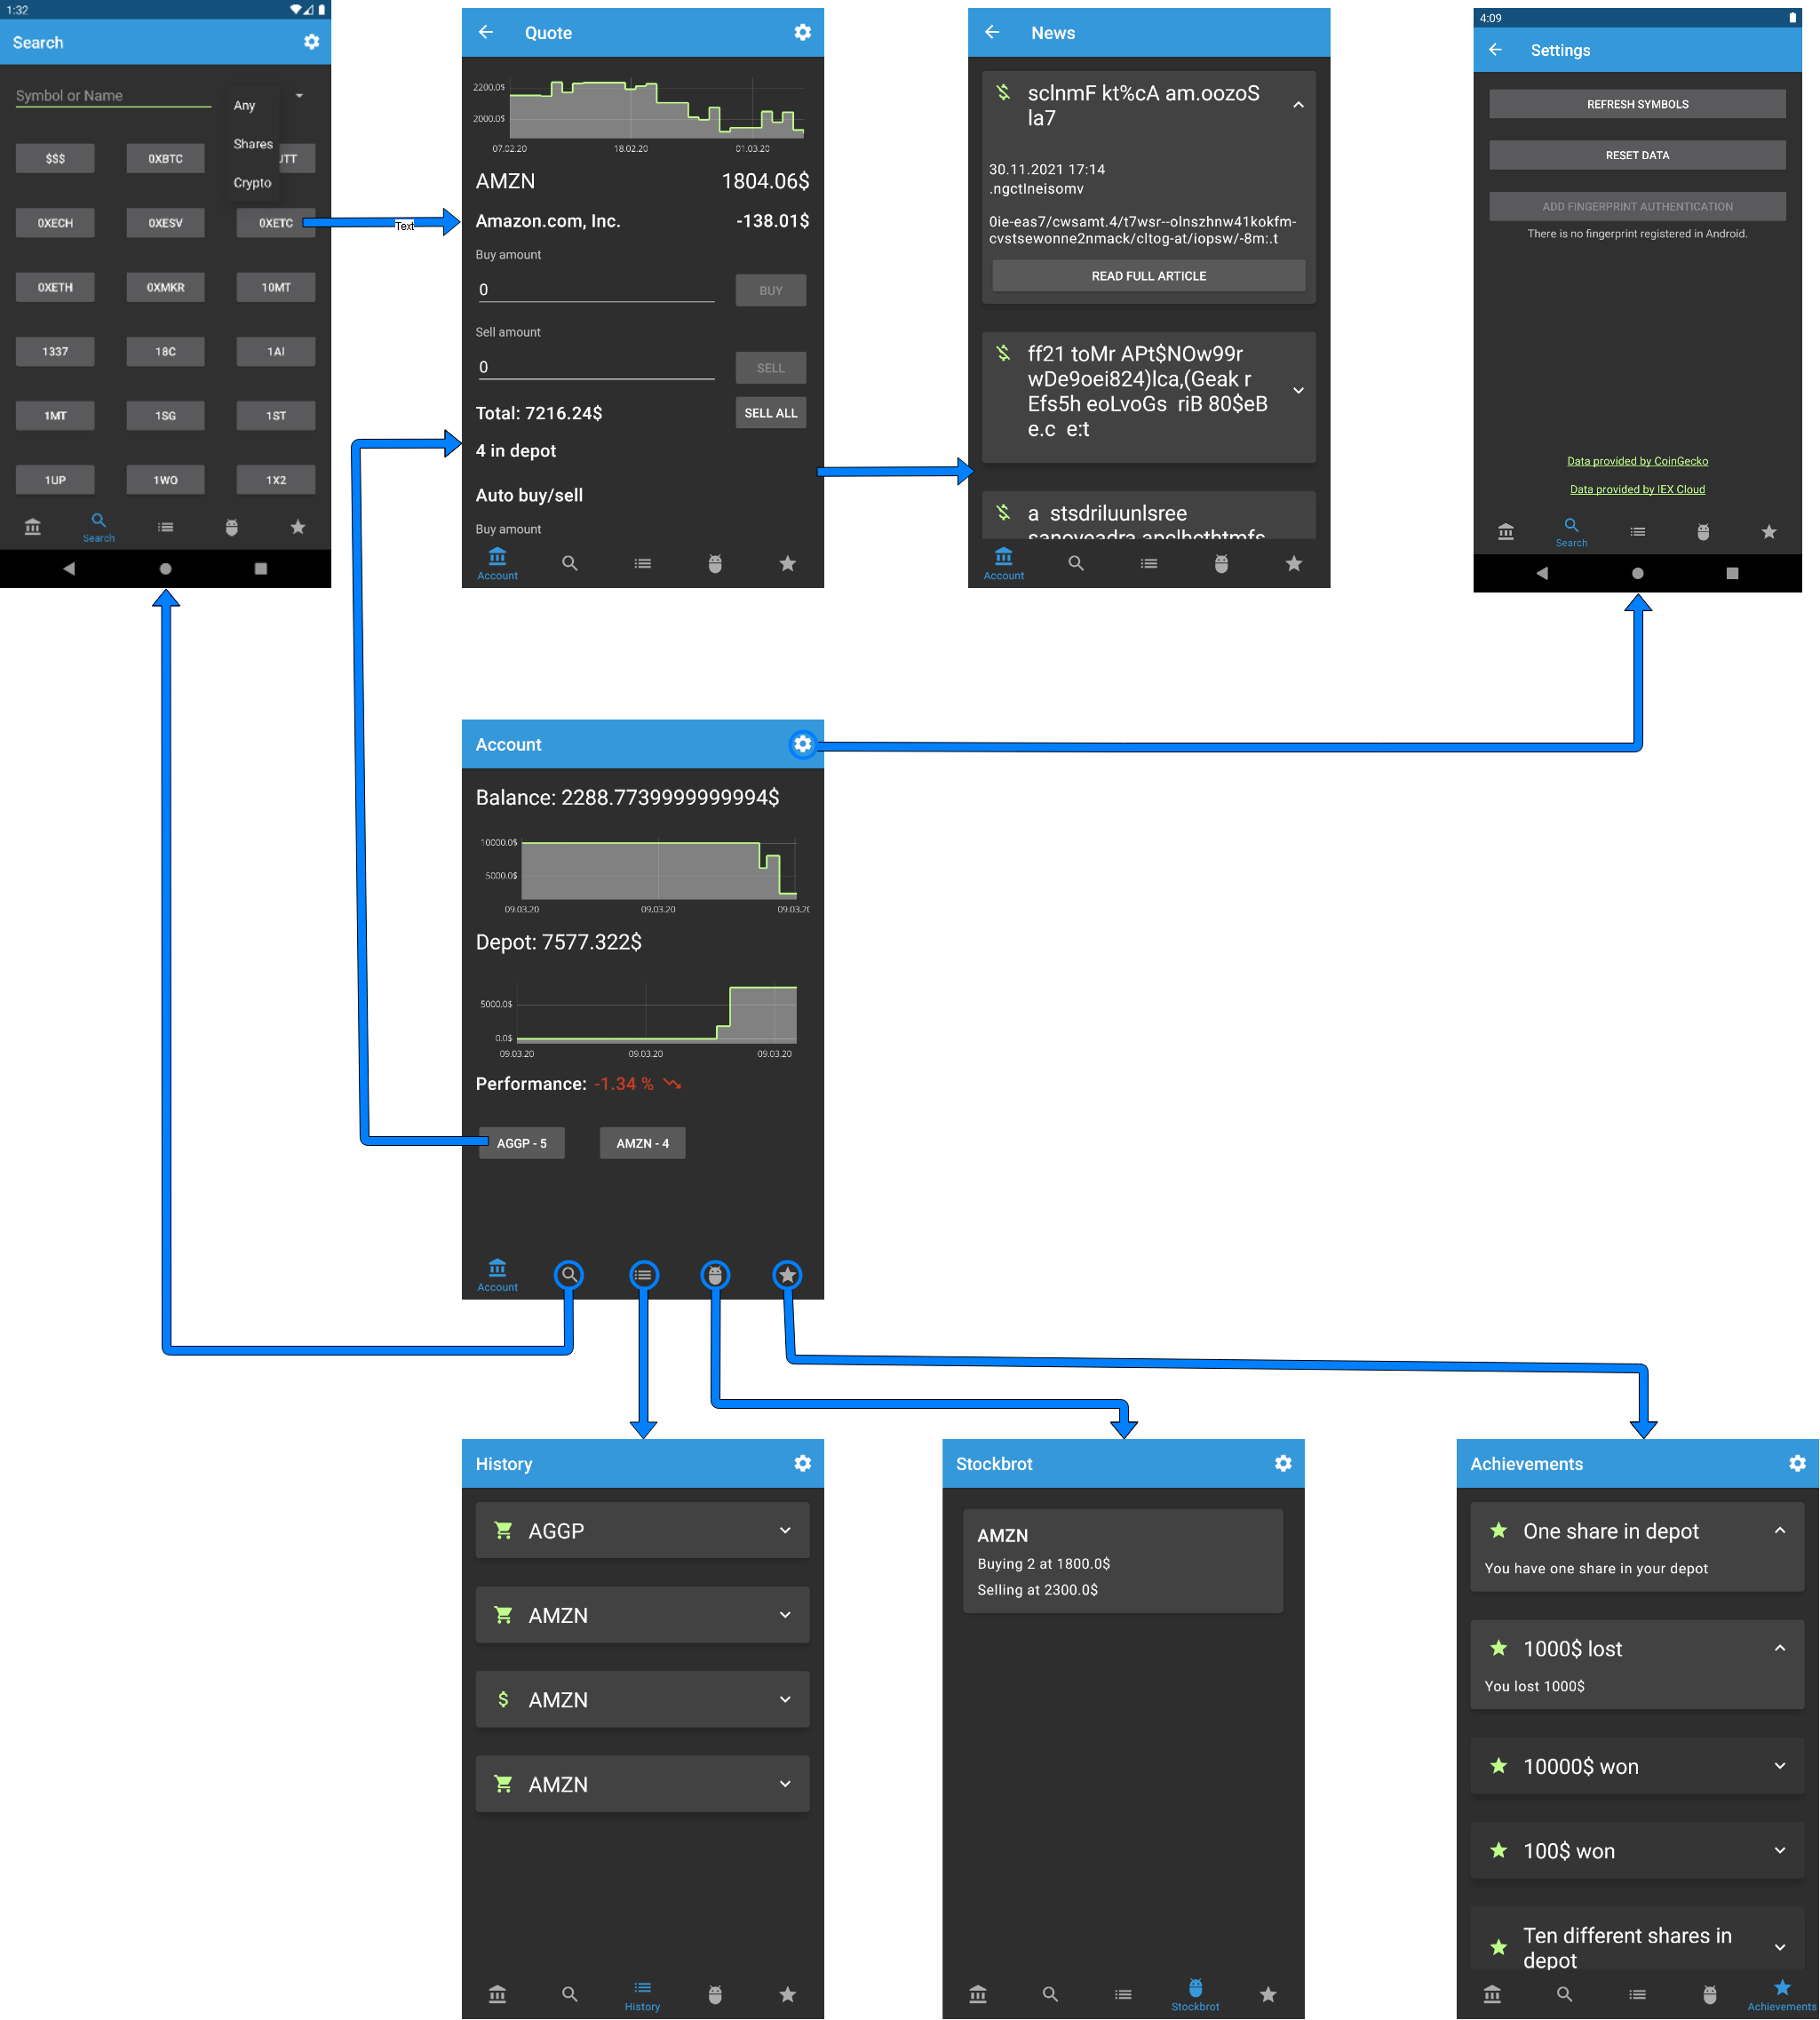
\includegraphics[height=12cm]{./images/navigation_screens/navigation_screens.png}
	\caption{Navigation zwischen den Bildschirmen}
	\label{fig:functionality:navigation:screens}
\end{figure}


\subsection{Account}
\label{subsec:functionality:account}
Im Account-Screen bekommt der Benutzer alle Informationen angezeigt, welche seinen Kontostand und sein Depot betreffen (siehe \autoref{fig:functionality:account}). Dieser Screen wird über den Eintrag "`Account"' in der Bottom Navigation erreicht.

Im oberen Teil des Bildschirms wird der aktuelle Kontostand in US-Dollar angezeigt. Darunter stellt ein Diagramm den Verlauf des Kontostands dar (siehe \autoref{fig:functionality:account:balance}).

Unter diesem Abschnitt wird der aktuelle Wert des Depots, sowie ein Diagramm über dessen Verlauf angezeigt (siehe \autoref{fig:functionality:account:depot}).

Die Performance des Gesamtdepots wird unter den Diagrammen angezeigt (siehe \autoref{fig:functionality:account:performance}). Sie misst, wie gut die Leistung des Investors war, das Startkapital zu vergrößern. Um diesen Wert deutlicher darzustellen, wird eine negative Performance in roter Schrift und einem absteigenden Pfeil, sowie eine positive Performance in grüner Schrift und einem aufsteigenden Pfeil gekennzeichnet.

Im letzten Abschnitt des Screens werden die bereits gekauften Anlagen aufgelistet (siehe \autoref{fig:functionality:account:depot_quotes}). Durch scrollen innerhalb der Ansicht, werden weitere Anlagen sichtbar, falls aus Platzgründen nicht alle unmittelbar sichtbar dargestellt werden können.

\begin{figure}[H]
    \begin{subfigure}{.5\textwidth}
        \centering
        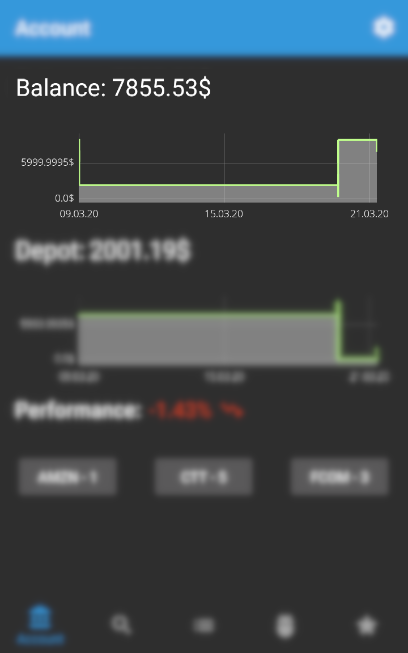
\includegraphics[height=8cm,keepaspectratio]{./images/account/balance.png}
        \caption{Kontostand und Verlauf}
        \label{fig:functionality:account:balance}
    \end{subfigure}
    \begin{subfigure}{.5\textwidth}
        \centering
        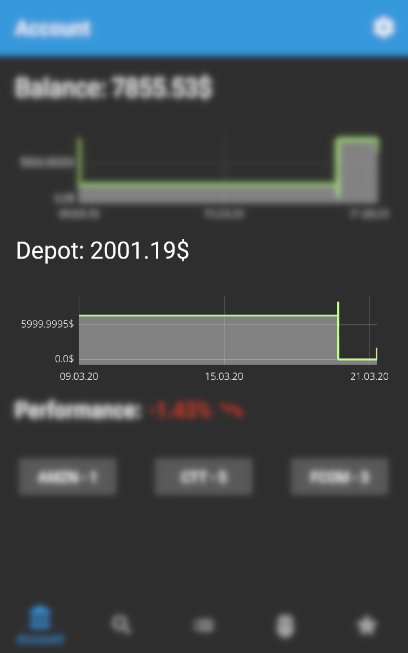
\includegraphics[height=8cm,keepaspectratio]{./images/account/depot.png}
        \caption{Depot und Verlauf}
        \label{fig:functionality:account:depot}
    \end{subfigure}
    \caption{Account}
    \label{fig:functionality:account}
\end{figure}

\begin{figure}[H]
    \ContinuedFloat
    \begin{subfigure}{.5\textwidth}
        \centering
        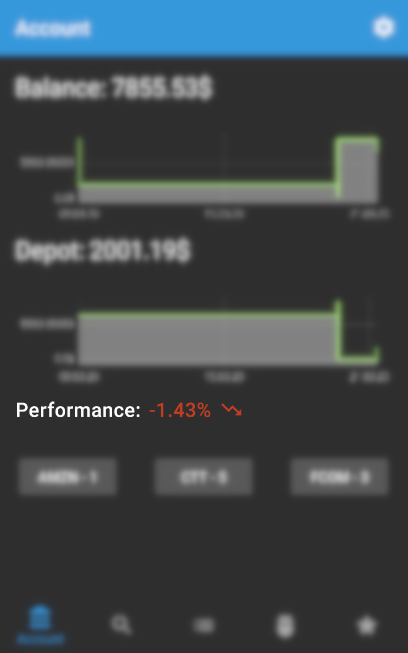
\includegraphics[height=8cm,keepaspectratio]{./images/account/performance.png}
        \caption{Performance}
        \label{fig:functionality:account:performance}
    \end{subfigure}
    \begin{subfigure}{.5\textwidth}
        \centering
        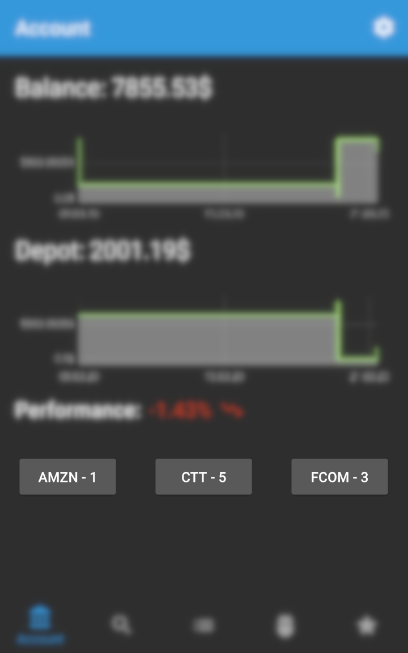
\includegraphics[height=8cm,keepaspectratio]{./images/account/depot_quotes.png}
        \caption{Anlagen im Depot}
        \label{fig:functionality:account:depot_quotes}
    \end{subfigure}
    \caption{Account (Fortsetzung)}
\end{figure}

Falls der Benutzer in den Einstellungen die Fingerabdrucks-Sperre aktiviert hat (siehe \autoref{fig:functionality:settings:fingerprint}), muss der Fingerabdruck nach dem Start der Anwendung bestätigt werden (siehe \autoref{fig:functionality:account:fingerprint:dialog}). Ohne diese Bestätigung ist es nicht möglich die Anwendung zu benutzen. Ein Abbruch des Authentifizierungsprozesses führt zum Schließen der App und zu einer Benachrichtigung über den entsprechenden Fehler (siehe \autoref{fig:functionality:account:fingerprint:cancel}). Selbiges gilt für die Durchführung der Authentifizierung mit einem nicht im Android-System hinterlegten Fingerabdruck (siehe \autoref{fig:functionality:account:fingerprint:failed}).

\begin{figure}[H]
    \begin{subfigure}{.329\textwidth}
        \centering
        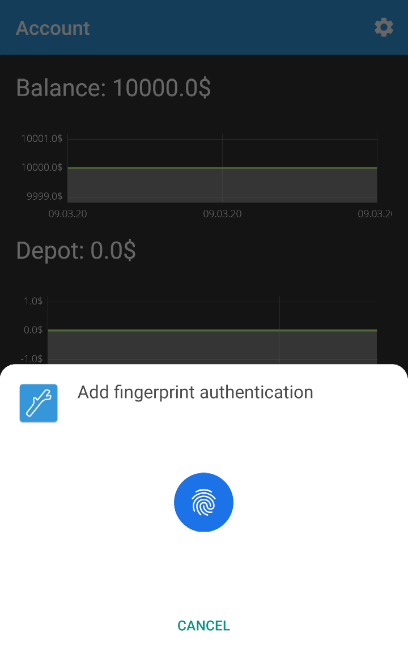
\includegraphics[height=6cm,keepaspectratio]{./images/account/fingerprint_required.png}
        \caption{Authentifizierung benötigt}
        \label{fig:functionality:account:fingerprint:dialog}
    \end{subfigure}
    \begin{subfigure}{.329\textwidth}
        \centering
        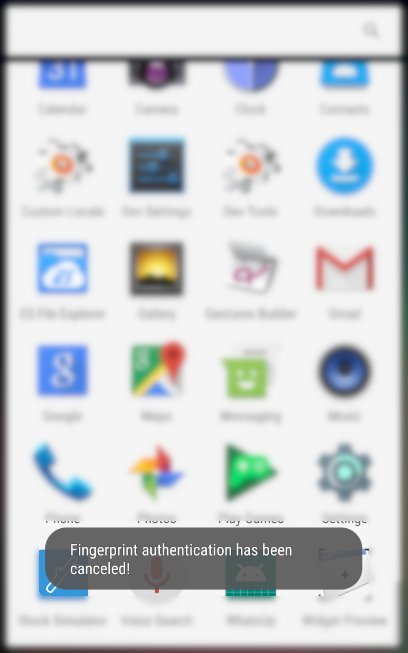
\includegraphics[height=6cm,keepaspectratio]{./images/account/fingerprint_required_cancel.png}
        \caption{Authentifizierung abgebrochen}
        \label{fig:functionality:account:fingerprint:cancel}
    \end{subfigure}
    \begin{subfigure}{.329\textwidth}
        \centering
        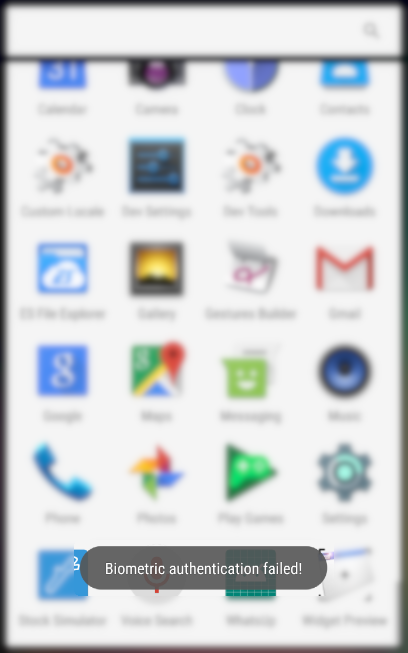
\includegraphics[height=6cm,keepaspectratio]{./images/account/fingerprint_required_wrong_finger.png}
        \caption{Authentifizierung fehlgeschlagen}
        \label{fig:functionality:account:fingerprint:failed}
    \end{subfigure}
    \caption{Fingerabdruck-Authentifizierung beim Anwendungsstart}
    \label{fig:functionality:account:fingerprint}
\end{figure}


\subsection{Suche}
\label{subsec:functionality:search}
Das Suchen von Aktien und Kryptowährungen nach Name und Symbol ist im Search-Screen möglich.
Zudem können Nutzer dort auswählen, ob sie nur Aktien, nur Kryptowährungen oder beide Anlagetypen sehen möchten.

Das Eingabefeld für Suchanfragen und die Dropdown-Liste zum Filtern befinden sich am oberen Bildschirmrand (siehe \autoref{fig:functionality:search:full}).
Darunter werden Suchergebnisse in einem scrollbaren Raster angezeigt (siehe \autoref{fig:functionality:search:results}).
Diese aktualisieren sich automatisch, sobald sich ein Suchkriterium verändert.
Dadurch ist es möglich, unmittelbar auf Nutzereingaben zu reagieren und Ergebnisse schnell anzuzeigen.
Während eine Suche stattfindet wird ein Fortschritts\-indikator angezeigt, um Nutzer über den aktuellen Zustand der Suche zu informieren (siehe \autoref{fig:functionality:search:loading}).
Sollte eine Suche keine Ergebnisse liefern wird eine entsprechende Meldung angezeigt (siehe \autoref{fig:functionality:search:no-results}).

Durch Klicken auf ein Suchergebnis können Nutzer zur Detailansicht dieses Anlageguts navigieren (siehe \autoref{subsec:functionality:quote}).

\begin{figure}[H]
	\begin{subfigure}{.5\textwidth}
		\centering
		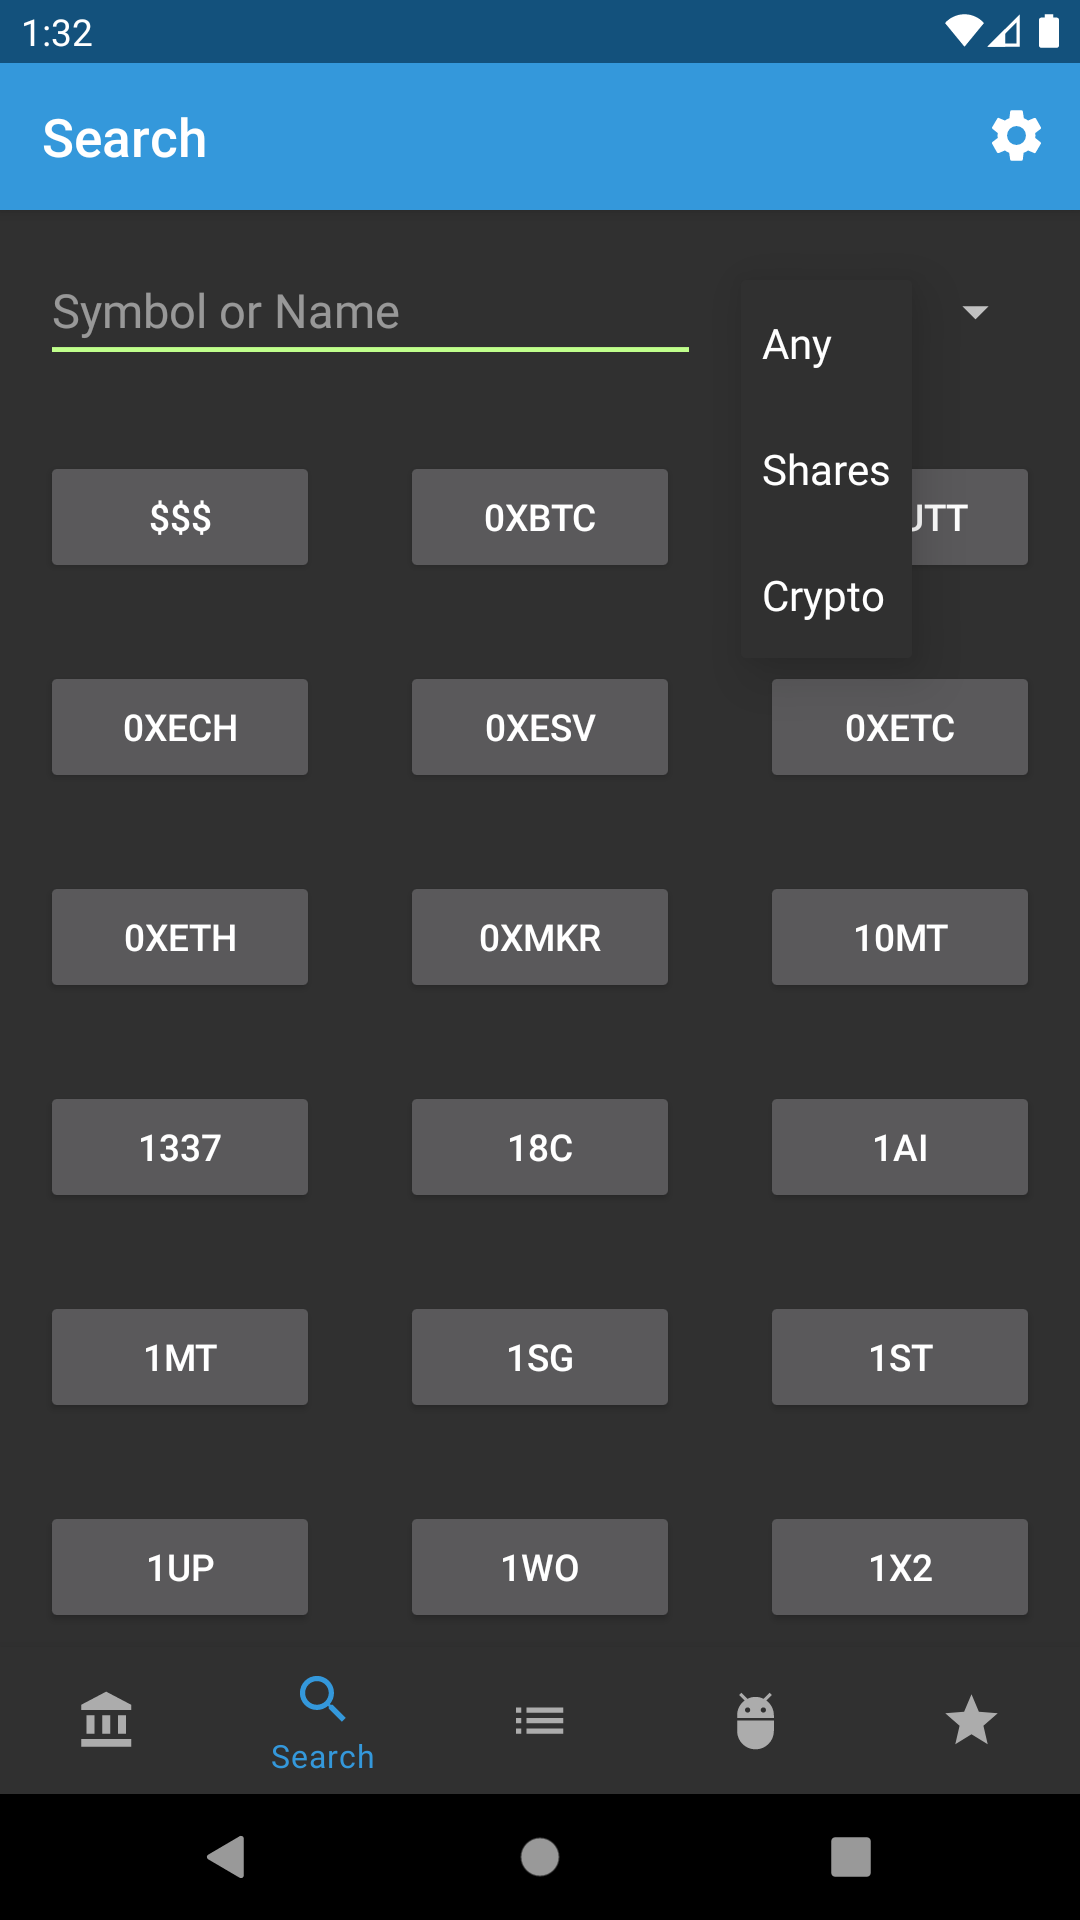
\includegraphics[height=8cm,keepaspectratio]{./images/search/type.png}
		\caption{Nutzereingabe}
		\label{fig:functionality:search:full}
	\end{subfigure}
	\begin{subfigure}{.5\textwidth}
		\centering
		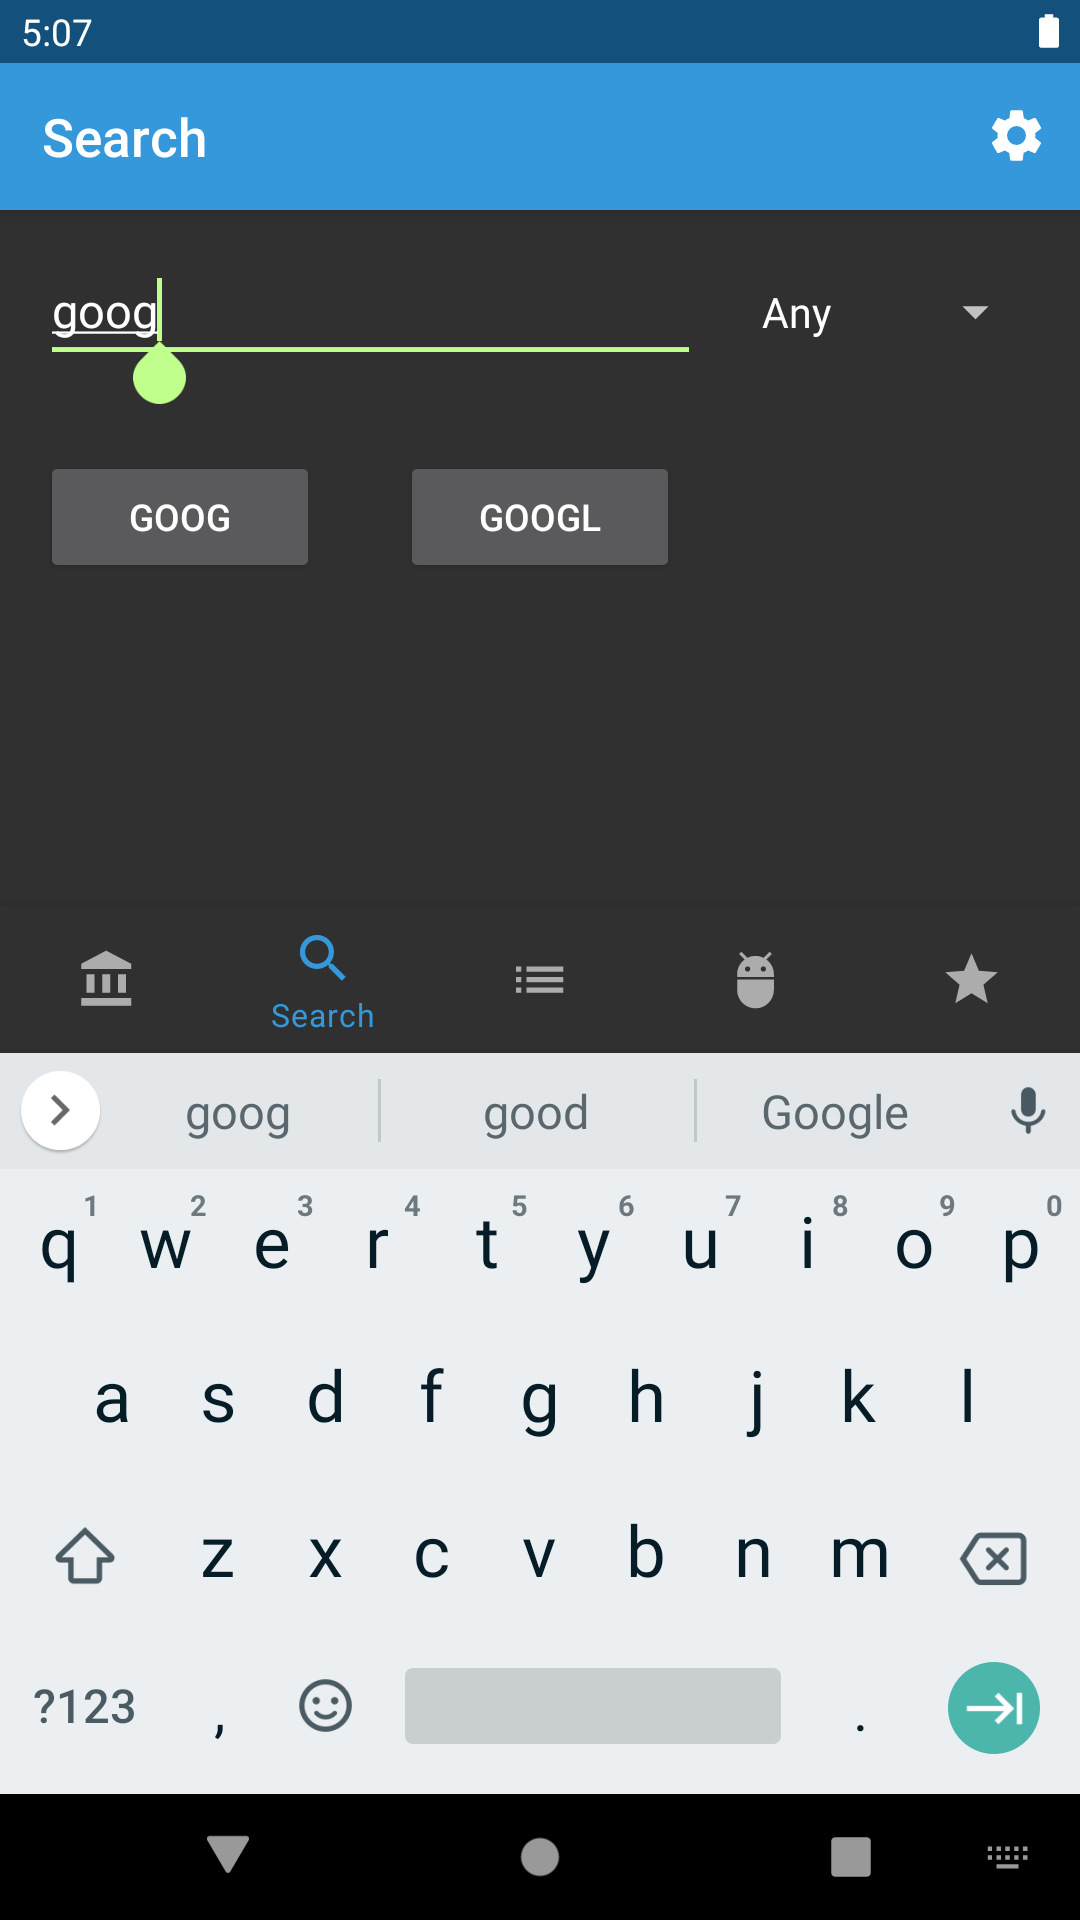
\includegraphics[height=8cm,keepaspectratio]{./images/search/done.png}
		\caption{Suchergebnisse}
		\label{fig:functionality:search:results}
	\end{subfigure}
	\begin{subfigure}{.5\textwidth}
		\centering
		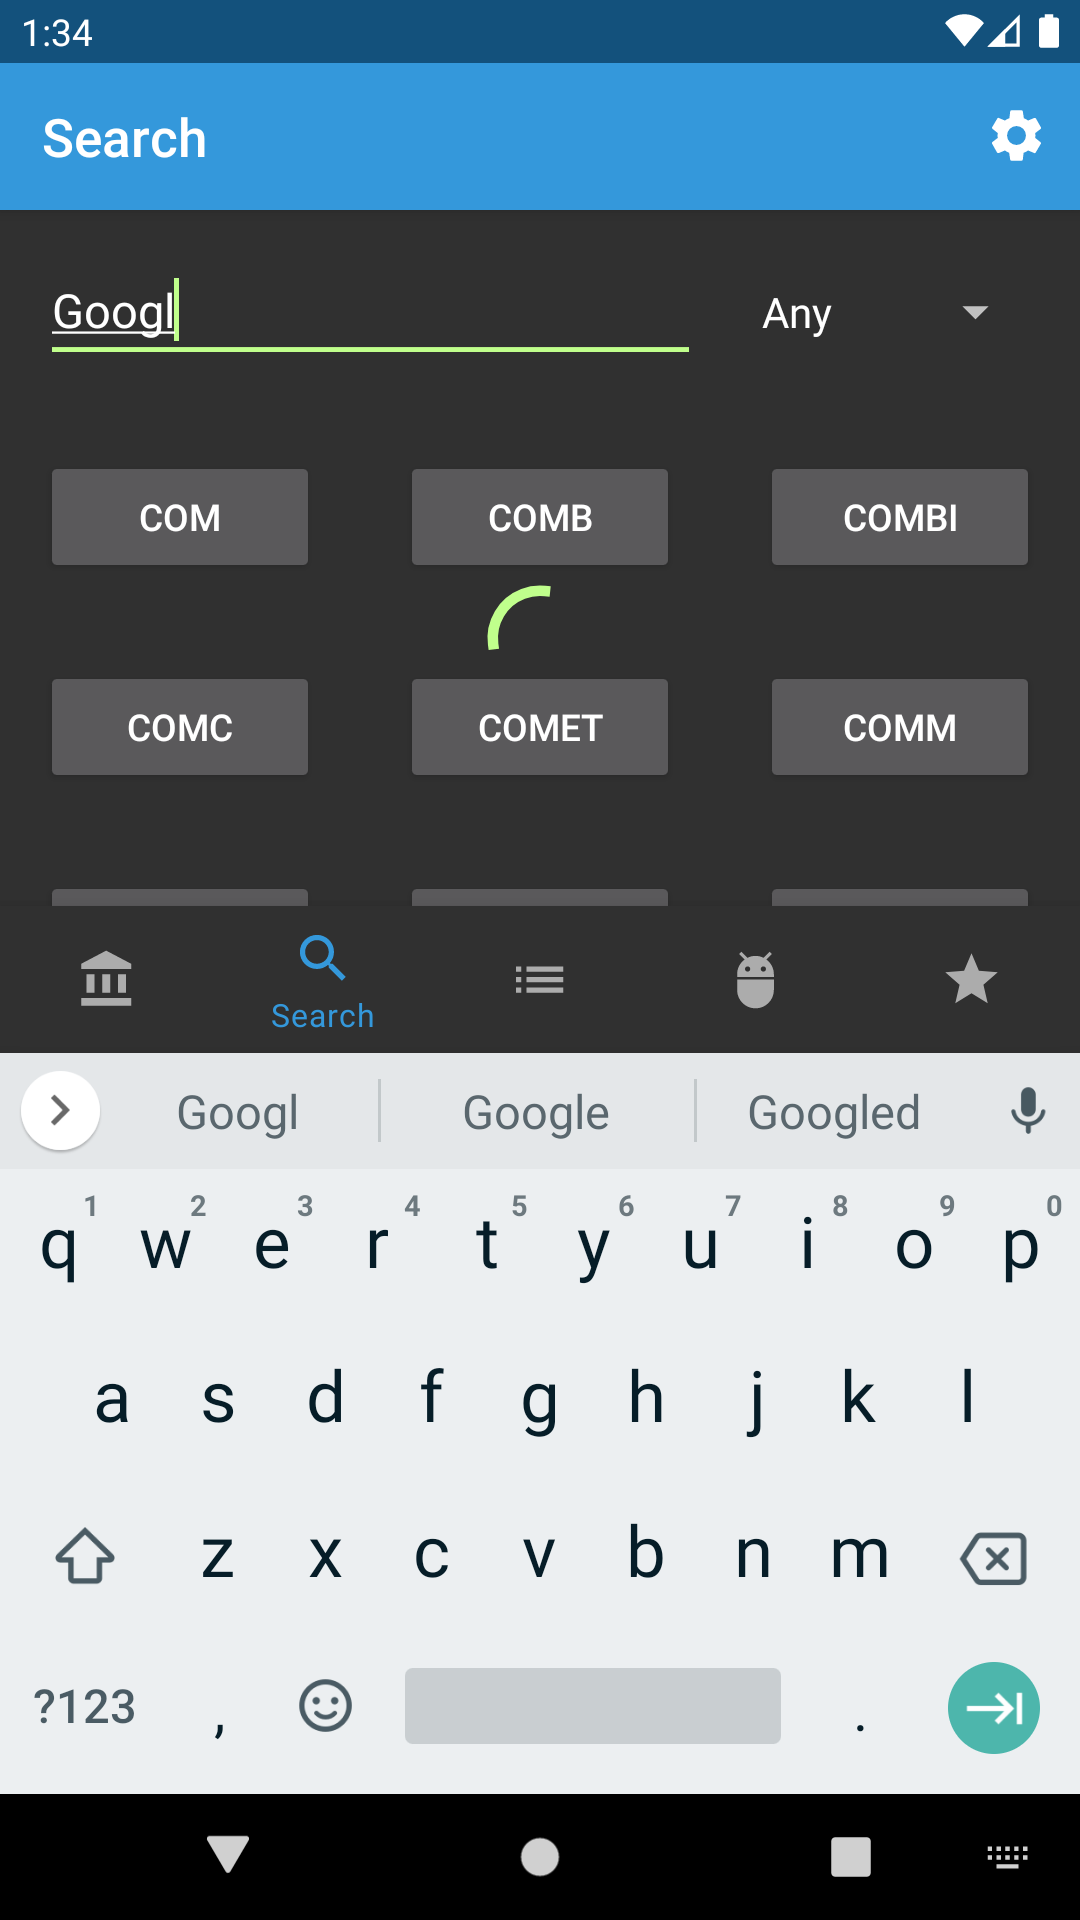
\includegraphics[height=8cm,keepaspectratio]{./images/search/loading.png}
		\caption{Fortschrittsindikator}
		\label{fig:functionality:search:loading}
	\end{subfigure}
	\begin{subfigure}{.5\textwidth}
		\centering
		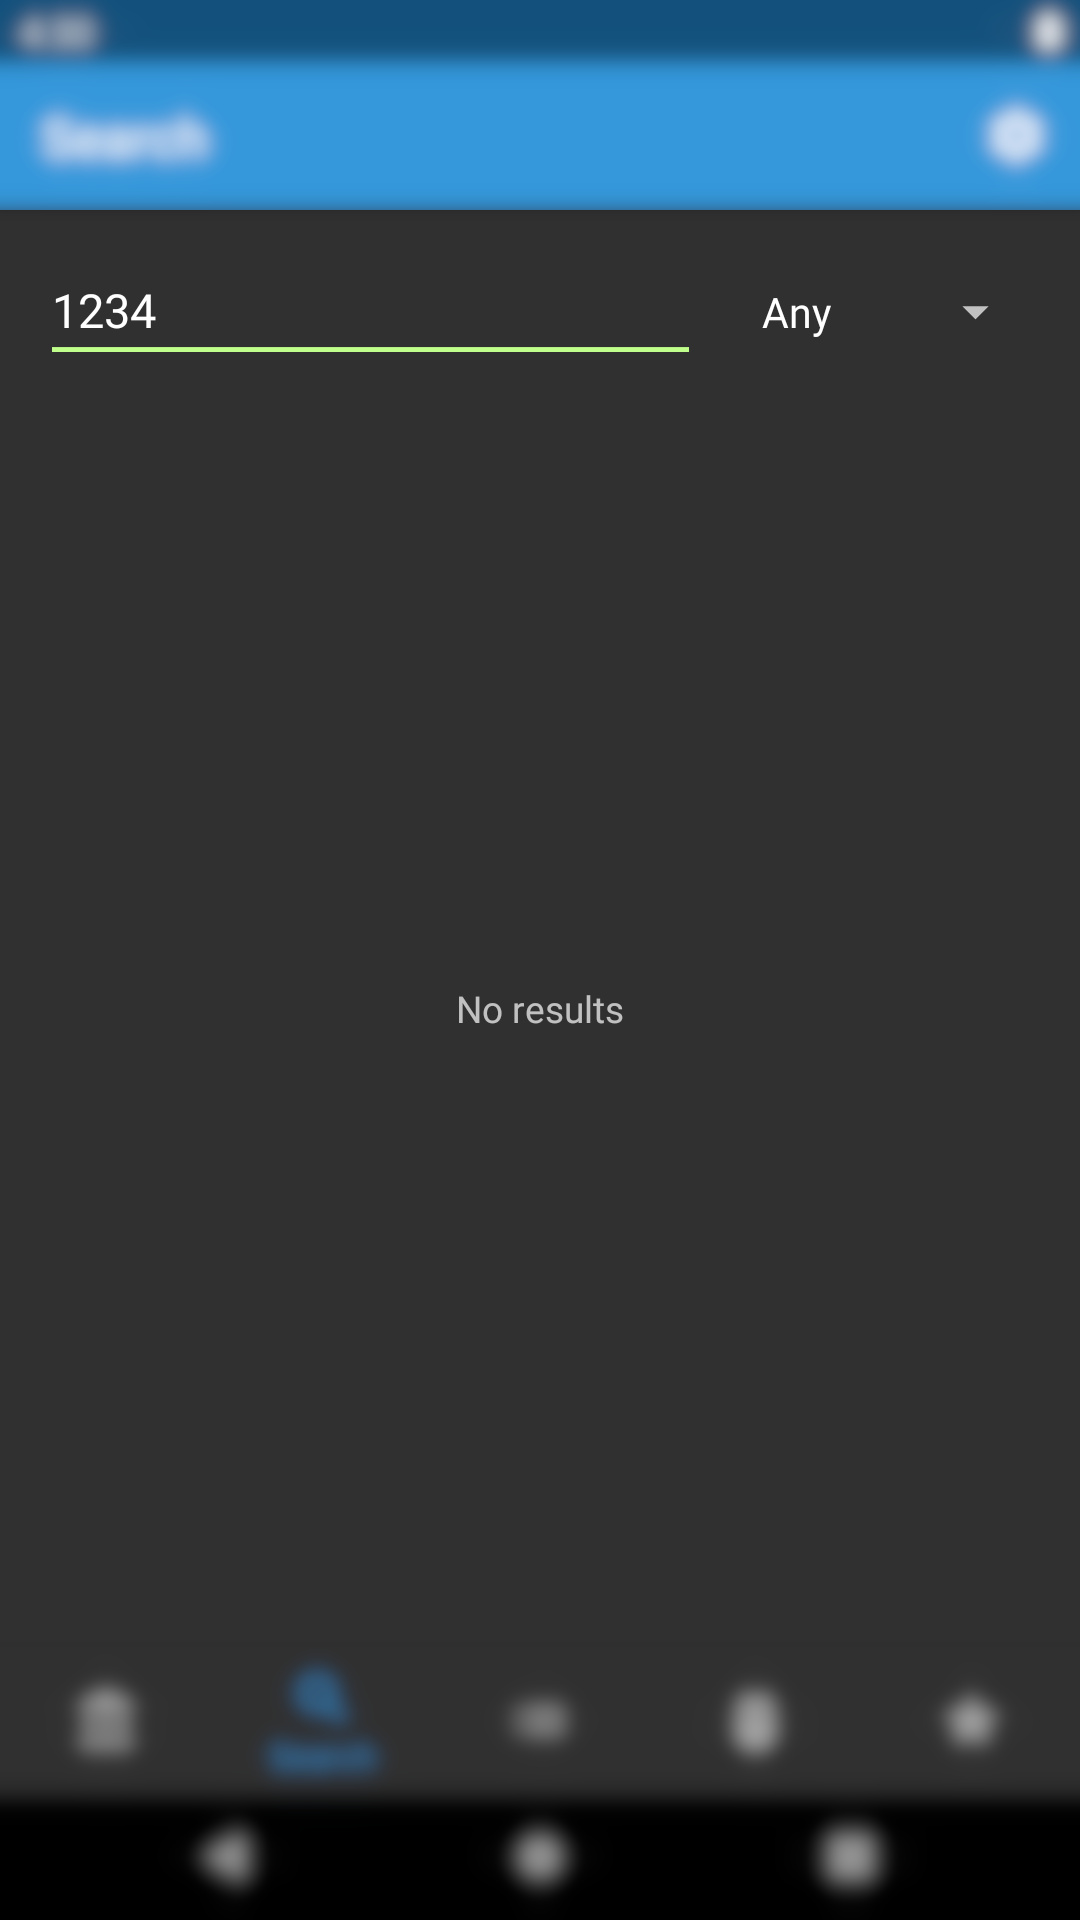
\includegraphics[height=8cm,keepaspectratio]{./images/search/no_results.png}
		\caption{Suche ohne Ergebnisse}
		\label{fig:functionality:search:no-results}
	\end{subfigure}
	\caption{Suche}
	\label{fig:functionality:search}
\end{figure}


\subsection{Transaktionshistorie}
\label{subsec:functionality:history}
Eine Übersicht über alle getätigten Transaktionen, das heißt Ein- und Verkäufe von Aktien und Kryptowährungen, werden im History-Screen dargestellt. Dieser wird über den Eintrag "`History"' der Bottom-Navigation erreicht. \autoref{fig:functionality:history:list_closed} zeigt den Aufbau des History-Screens. Transaktionen werden in Form von ausklappbaren Karten dargestellt.

\begin{figure}[H]
	\centering
    \begin{subfigure}{.49\textwidth}
        \centering
        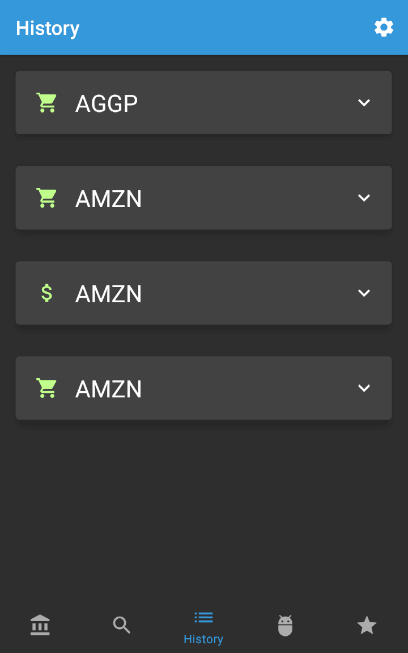
\includegraphics[height=8cm,keepaspectratio]{./images/history_list.png}
        \caption{geschlossen}
        \label{fig:functionality:history:list_closed}
    \end{subfigure}
    \begin{subfigure}{.49\textwidth}
        \centering
        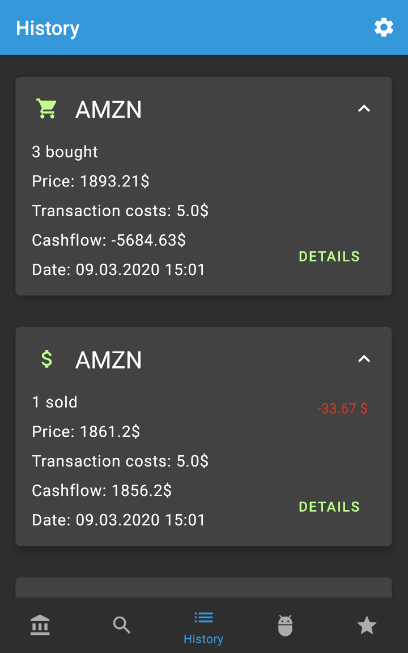
\includegraphics[height=8cm,keepaspectratio]{./images/history_list_open.png}
        \caption{geöffnet}
        \label{fig:functionality:history:list_open}
    \end{subfigure}
	\caption{Historie}
	\label{fig:functionality:history:list}
\end{figure}

Die Karten sind nach dem Zeitpunkt ihrer Durchführung absteigend geordnet, sodass die jüngste Transaktion zu Beginn positioniert ist. Eine Karte beinhaltet das Symbol der jeweiligen Anlage und ein Icon, mit dem angezeigt wird, ob es sich bei der Transaktion um einen Kauf (Einkaufswagen) oder einen Verkauf (Dollar-Symbol) handelt. Durch Klick auf den Pfeil kann eine Transaktionskarte ausgeklappt werden, um die Details der jeweiligen Transaktion anzuzeigen (siehe \autoref{fig:functionality:history:list_open}). In der Detailansicht wird angezeigt, wie viele Anlagen ge- oder verkauft wurden, der Preis dieser Anlage zum Zeitpunkt der Transaktion, die Transaktionskosten, der dadurch bewirkte Geldfluss (Cashflow) sowie das Datum und die Uhrzeit, zu der die Transaktion durchgeführt wurde. Zusätzlich wird bei einem Verkauf angezeigt, wie hoch der Gewinn bzw. Verlust durch diesen Verkauf war.


\subsection{Stockbrot}
\label{subsec:functionality:stockbrot}
Der Name Stockbrot ist ein Wortspiel aus den Begriffen stock (deutsch: Aktie) und Bot, die Kurzform von robot (deutsch: Roboter). Mithilfe dieses Bots ist der Benutzer in der Lage das Traden von Aktien oder Kryptowährungen zu automatisieren. Für jede Anlage, welche sich unter der Kontrolle des Bots befindet, wird alle 15 Minuten ein sogenannter \textit{Worker} ausgeführt (siehe \autoref{subsubsec:technologies:bibs:workmanager}). Vom Worker wird geprüft, ob die zuvor in der Detailansicht (\autoref{subsec:functionality:quote}) festgelegten Schwellwerte des jeweiligen aktuellen Kurses erreicht wurden. Falls dies der Fall ist, wird eine entsprechende Transaktion ausgeführt. Die Worker werden im Hintergrund mithilfe des \textit{WorkManagers} gesteuert (siehe \autoref{subsubsec:technologies:bibs:workmanager}).

\autoref{fig:functionality:stockbrot:overview} zeigt den Screen, der eine Übersicht über die von Stockbrot verwalteten Aktien und Kryptowährungen liefert. Die Navigation zu diesem Screen erfolgt über einen Klick auf den Eintrag "`Stockbrot"' in der Bottom Navigation. Wenn zuvor keine Aktien oder Kryptowährungen zu dem Bot hinzugefügt wurden, werden in diesem Screen keine Einträge aufgelistet (\autoref{fig:functionality:stockbrot:overview:empty}). Sobald eine Anlage der Kontrolle des Bots über die Detailansicht einer Anlage (\autoref{subsec:functionality:quote}) übergeben wurde, wird diese als Element der Liste angezeigt (\autoref{fig:functionality:stockbrot:overview:entry}). Jedes dieser Elemente besteht aus der Id, sowie den Schwellwerten, bei deren Unter- oder Überschreitung der Bot einen Kauf- oder Verkauf veranlassen soll. Zusätzlich zu dem Schwellwert für automatische Käufe, wird die Anzahl der maximal zu kaufenden Anlagen dargestellt. Für Verkäufe existiert ein solches Limit nicht, weshalb es in den Elementen auch nicht dargestellt wird.

\begin{figure}[H]
    \begin{subfigure}{.5\textwidth}
        \centering
        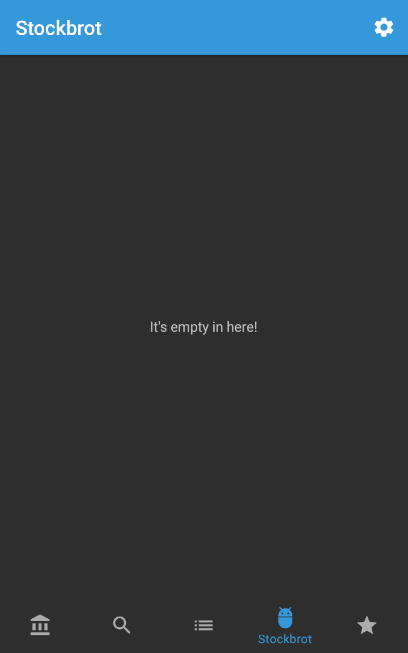
\includegraphics[height=8cm,keepaspectratio]{./images/stockbrot_list_empty.png}  
        \caption{Stockbrot Übersicht ohne Eintrag}
        \label{fig:functionality:stockbrot:overview:empty}
    \end{subfigure}
    \begin{subfigure}{.5\textwidth}
        \centering
        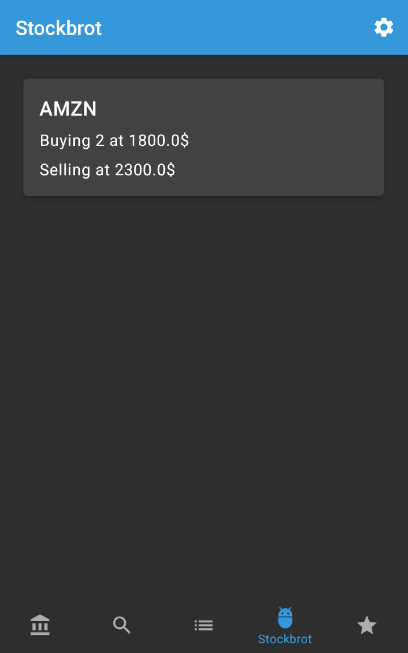
\includegraphics[height=8cm,keepaspectratio]{./images/stockbrot_list.png}  
        \caption{Stockbrot Übersicht mit Eintrag}
        \label{fig:functionality:stockbrot:overview:entry}
    \end{subfigure}
    \caption{Stockbrot Übersicht}
    \label{fig:functionality:stockbrot:overview}
\end{figure}


\subsection{Errungenschaften}
\label{subsec:functionality:achievements}
Um den Benutzer des Spiels vor Herausforderungen zu stellen und damit den Spielspaß zu erhöhen, sind verschiedene Errungenschaften erreichbar. Eine Übersicht über diese Erfolge, sind im Achievements-Screen einsehbar, welcher über den Eintrag "`Achievements"' in der Bottom Navigation zu erreichen ist. Dieser Screen listet, wie in \autoref{fig:functionality:achievements:overview:closed} sichtbar, alle bereits erreichten und noch freizuschaltenden Errungenschaften auf. Die Hintergrundfarben der noch nicht freigeschalteten Errungenschaften, werden in der Liste ausgegraut. Jedes der Elemente besteht aus einem Titel und einer Beschreibung. Die Beschreibung ist für alle bereits erreichten Errungenschaften, mittels Pfeil auf der rechten Seite des Elements, aufklappbar (\autoref{fig:functionality:achievements:overview:open}).

\begin{figure}[H]
    \begin{subfigure}{.5\textwidth}
        \centering
        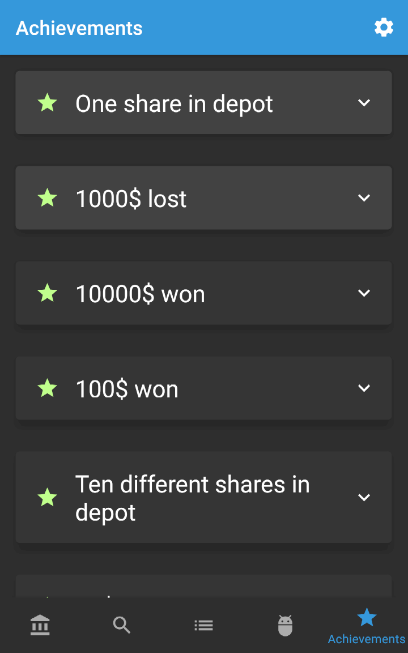
\includegraphics[height=8cm,keepaspectratio]{./images/achievements_list.png}  
        \caption{Errungenschaften Übersicht ohne Beschreibung}
        \label{fig:functionality:achievements:overview:closed}
    \end{subfigure}
    \begin{subfigure}{.5\textwidth}
        \centering
        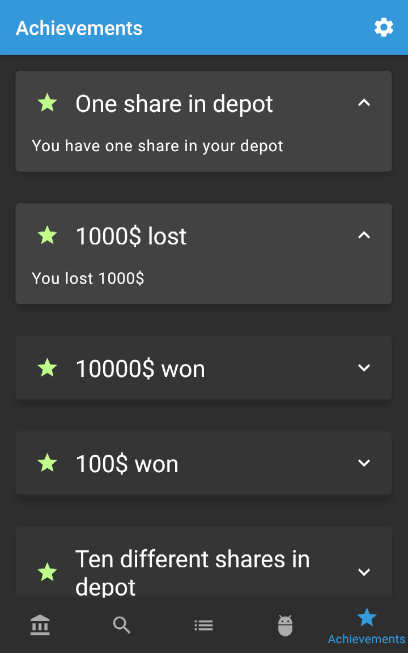
\includegraphics[height=8cm,keepaspectratio]{./images/achievements_list_open.png}  
        \caption{Errungenschaften Übersicht mit Beschreibung}
        \label{fig:functionality:achievements:overview:open}
    \end{subfigure}
    \caption{Errungenschaften Übersicht}
    \label{fig:functionality:achievements:overview}
\end{figure}

Sobald eine Errungenschaft freigeschaltet wird, erscheint im unteren Teil des aktuellen Screens eine Toast-Benachrichtigung \autocite{android_toasts} (siehe \autoref{fig:functionality:achievements:reached}). Diese zeigt den Titel der Errungenschaft an. Beim nächsten Aufruf der Übersicht der Errungenschaften ist dieser soeben erreichte Erfolg nicht mehr ausgegraut und die Beschreibung lässt sich einsehen. Sollten mehrere Errungenschaften direkt hintereinander freigeschaltet werden, werden auch die Benachrichtigungen nacheinander angezeigt. Intern wird sichergestellt, dass kein Erfolgt mehrfach angezeigt wird, selbst wenn die Kriterien zur Freischaltung eines Erfolgs öfter erfüllt werden.

\begin{figure}[H]
    \centering
    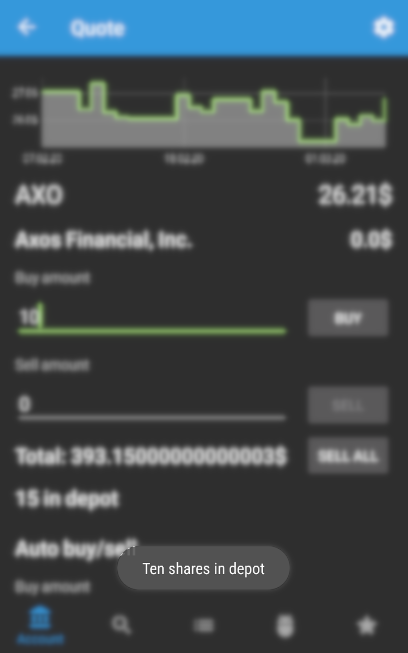
\includegraphics[height=8cm,keepaspectratio]{./images/achievement_reached.png}
    \caption{Errungenschaft wurde erreicht}
    \label{fig:functionality:achievements:reached}
\end{figure}


\subsection{Detailansicht}
\label{subsec:functionality:quote}
In der Detailansicht sind allgemeine Informationen über ein Anlagegut zu sehen (siehe \autoref{fig:functionality:quote:information}).
Dazu zählen Symbol, Name, aktueller Kurs und Kursänderung des Anlageguts.
Sollten keine Informationen über Kursänderungen vorliegen, wird stattdessen "`N/D"' angezeigt.

Darüber wird der Kursverlauf des Anlageguts angezeigt (siehe \autoref{fig:functionality:quote:history}).
Auch hier werden Platzhalter verwendet, falls keine Daten vorliegen.

\begin{figure}[H]
	\begin{subfigure}{.5\textwidth}
		\centering
		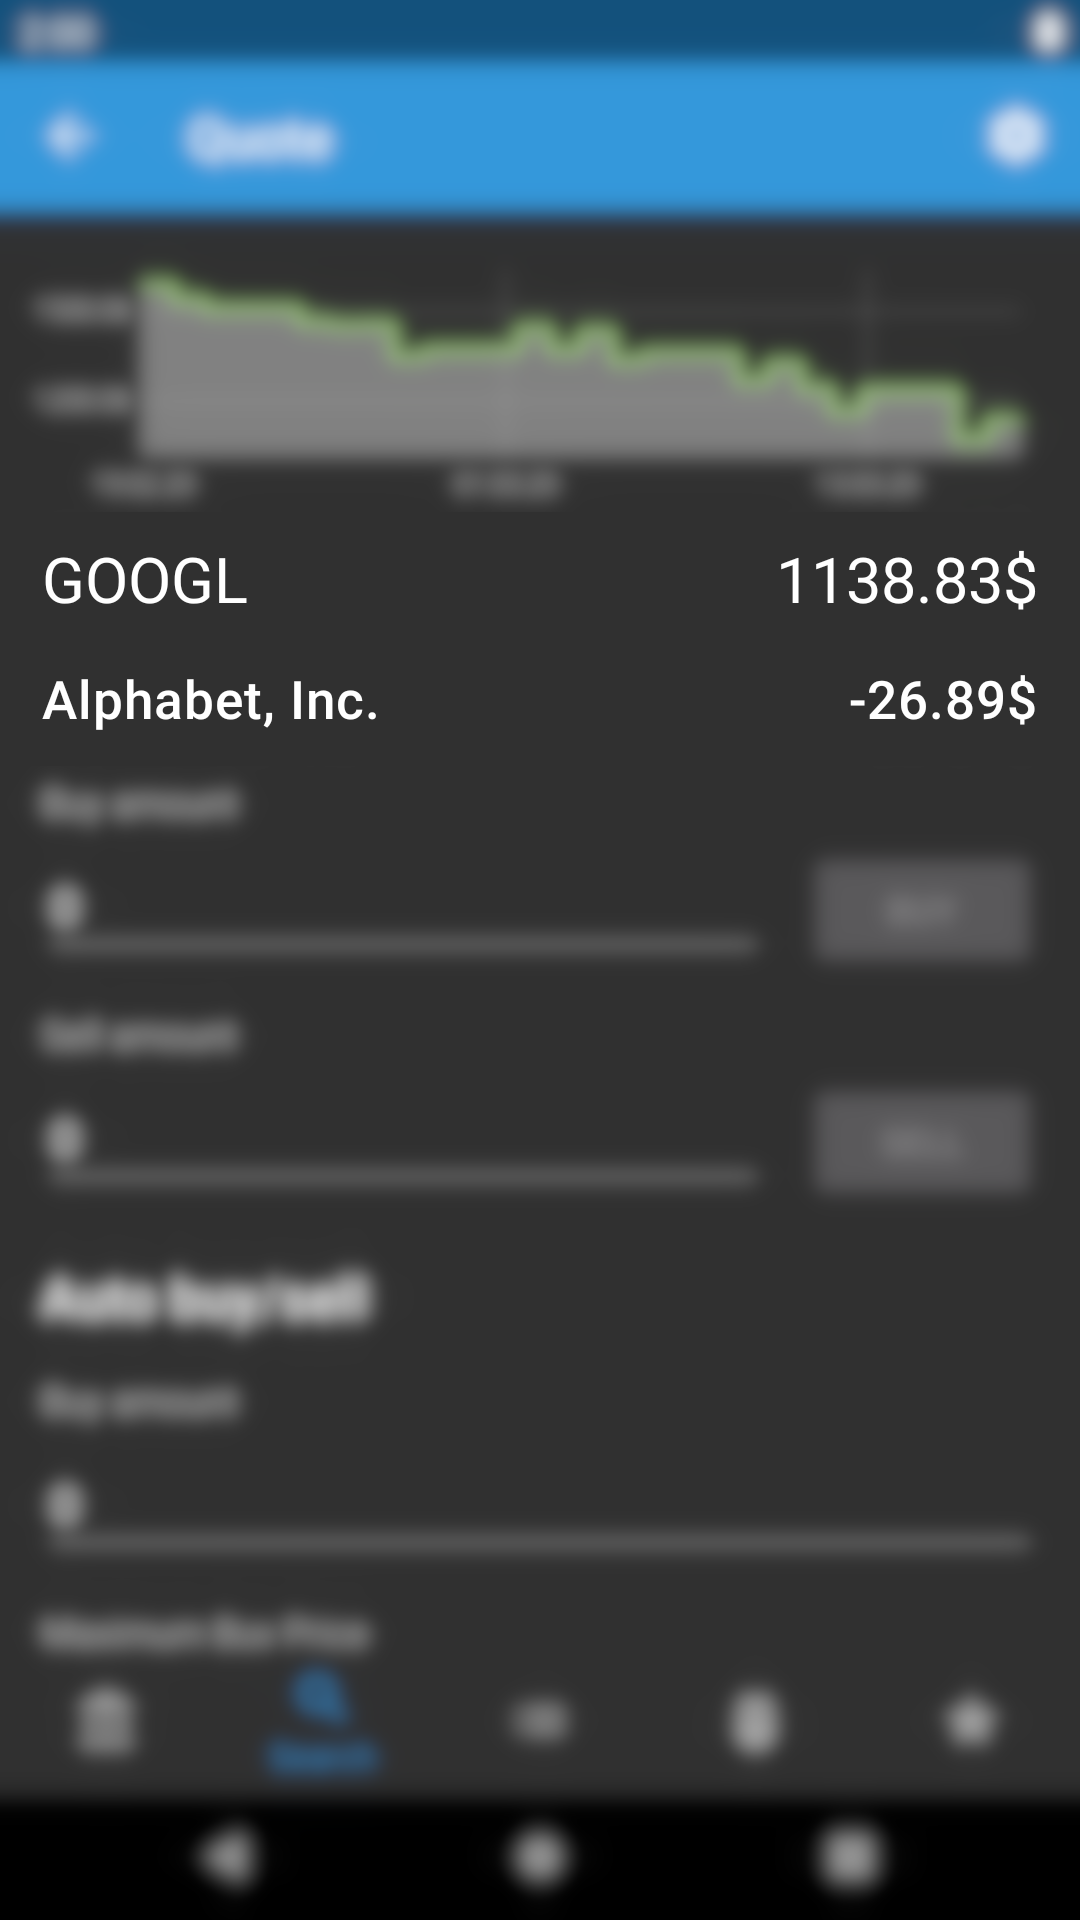
\includegraphics[height=8cm,keepaspectratio]{./images/quote/information.png}
		\caption{Informationen}
		\label{fig:functionality:quote:information}
	\end{subfigure}
	\begin{subfigure}{.5\textwidth}
		\centering
		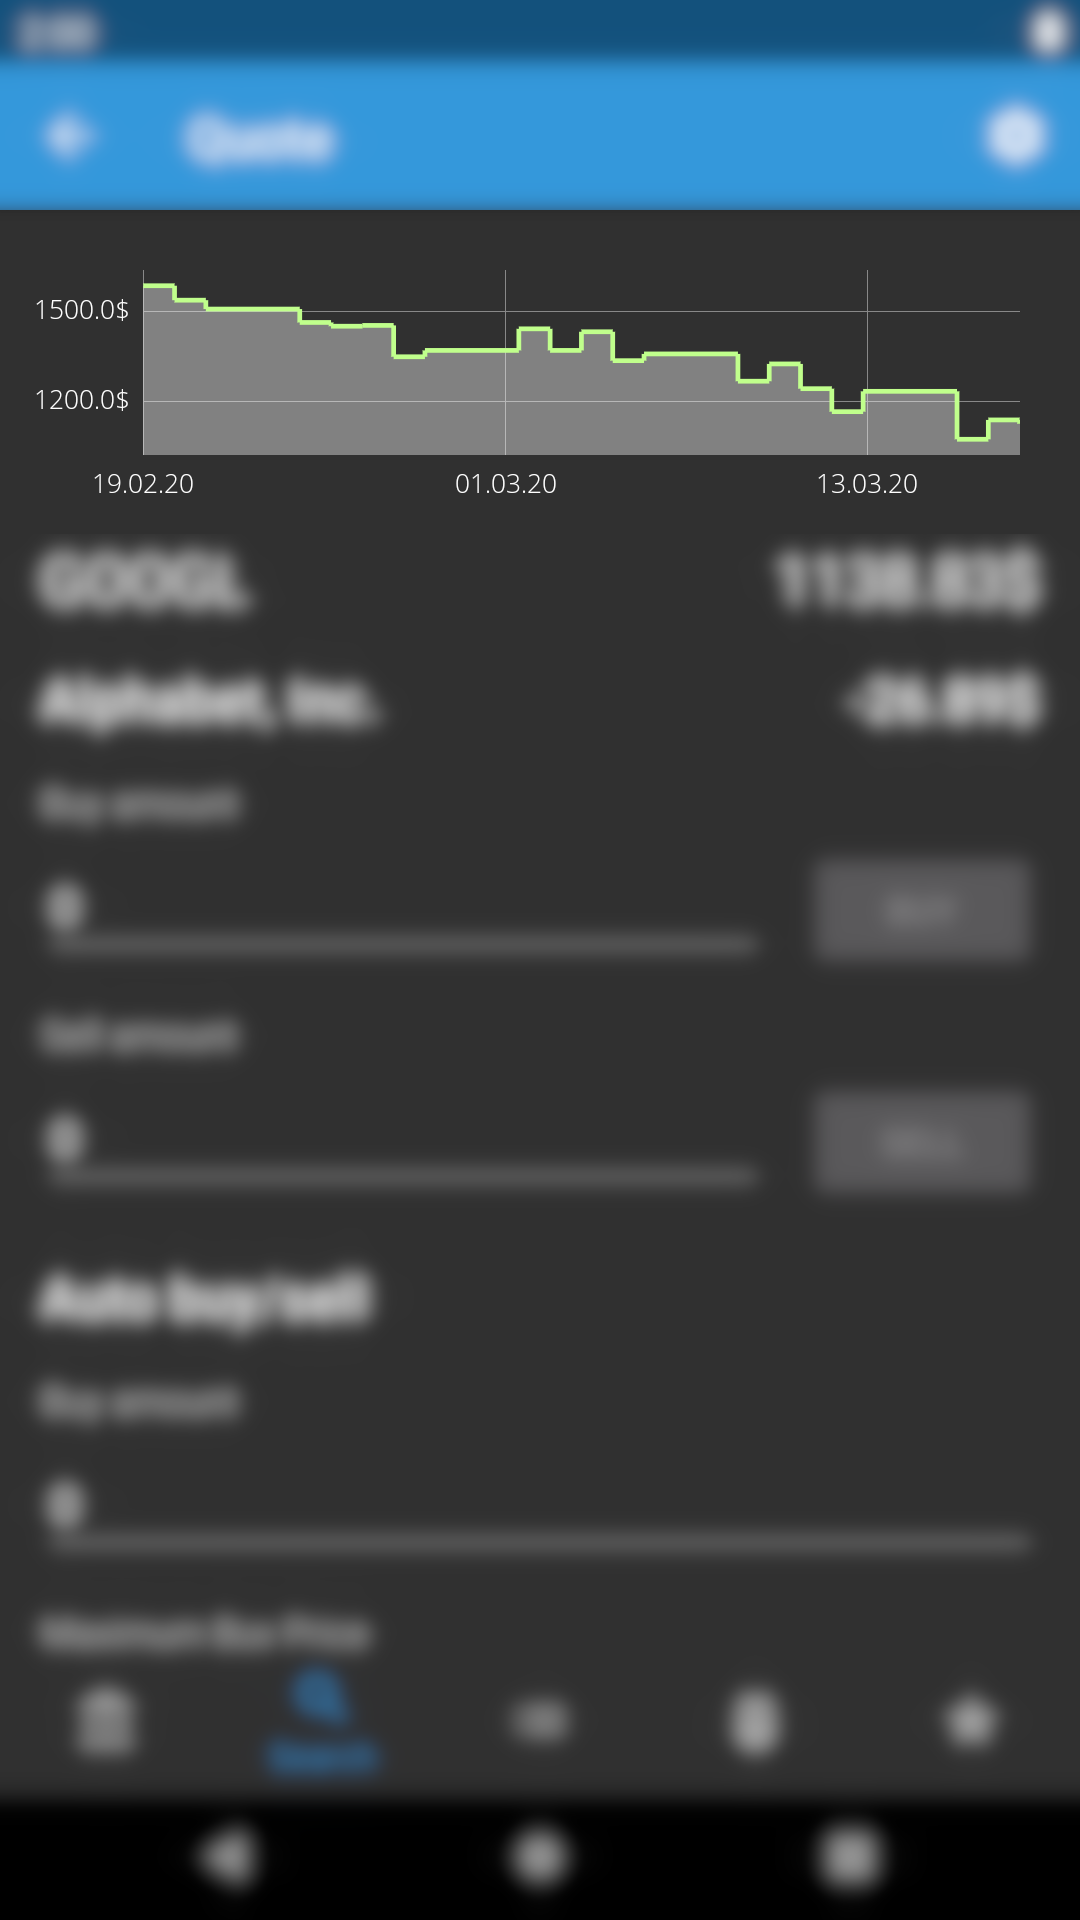
\includegraphics[height=8cm,keepaspectratio]{./images/quote/history.png}
		\caption{Kursverlauf}
		\label{fig:functionality:quote:history}
	\end{subfigure}
	\caption{Detailansicht}
	\label{fig:functionality:quote}
\end{figure}

Kaufen und Verkaufen findet über separate Eingabefelder statt (siehe \autoref{fig:functionality:buy-sell:input}).
Die zugehörigen Buttons sind nur aktiviert, wenn die Eingabe einen Kauf beziehungsweise Verkauf zulässt.

Nach Betätigen eines Buttons müssen Nutzer die Transaktion noch einmal bestätigen.
Dafür wird ein Bestätigungsdialog geöffnet (siehe \autoref{fig:functionality:buy-sell:dialog}), der die Transaktionsinformationen zudem erneut anzeigt.

Haben Nutzer ein Anlagegut im Depot, wird dies ebenfalls in der Detailansicht vermerkt (siehe \autoref{fig:functionality:buy-sell:in-depot}).
Es werden sowohl die Menge als auch der Gesamtwert angezeigt.
Zusätzlich wird der Button "`SELL ALL"' aktiviert, welcher einen kompletten Ausverkauf des entsprechenden Anlageguts aus dem Depot durchführt.

\begin{figure}[H]
	\begin{subfigure}{.5\textwidth}
		\centering
		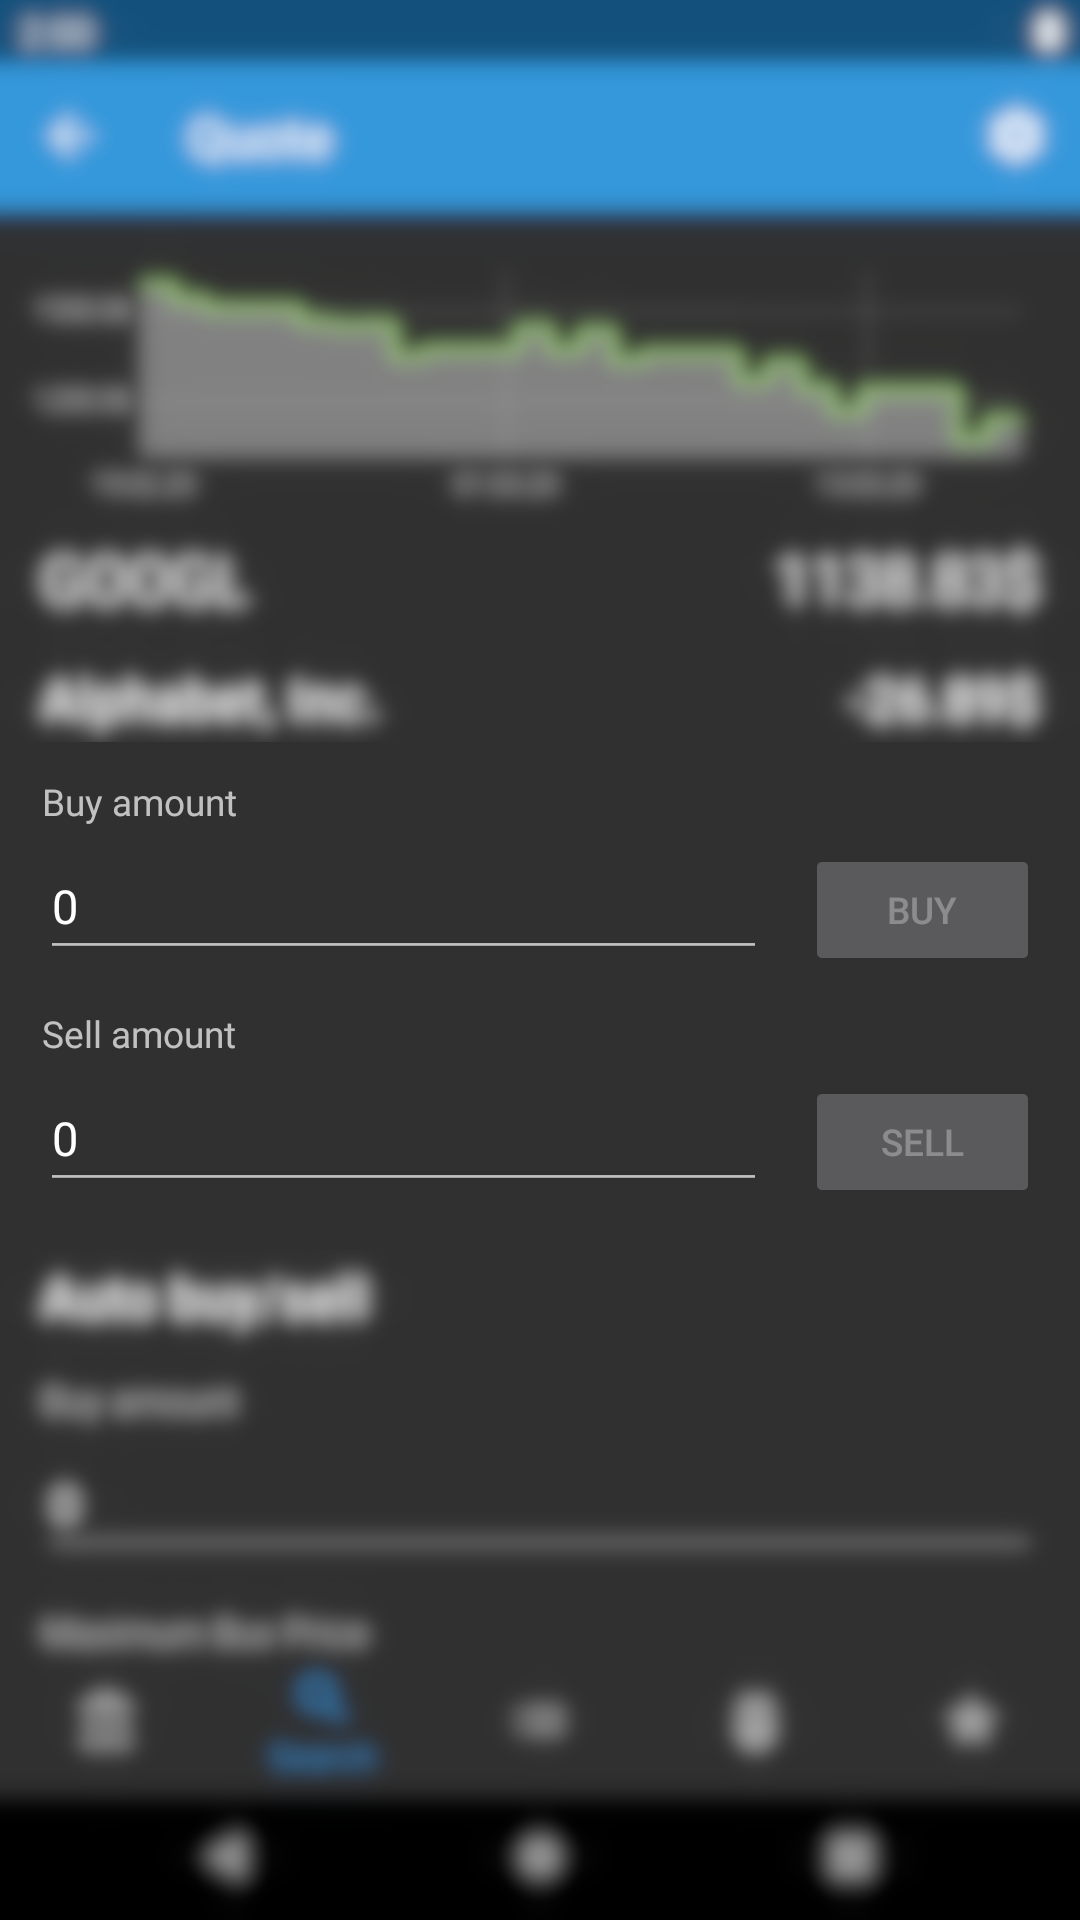
\includegraphics[height=8cm,keepaspectratio]{./images/quote/buy_sell.png}
		\caption{Nutzereingabe}
		\label{fig:functionality:buy-sell:input}
	\end{subfigure}
	\begin{subfigure}{.5\textwidth}
		\centering
		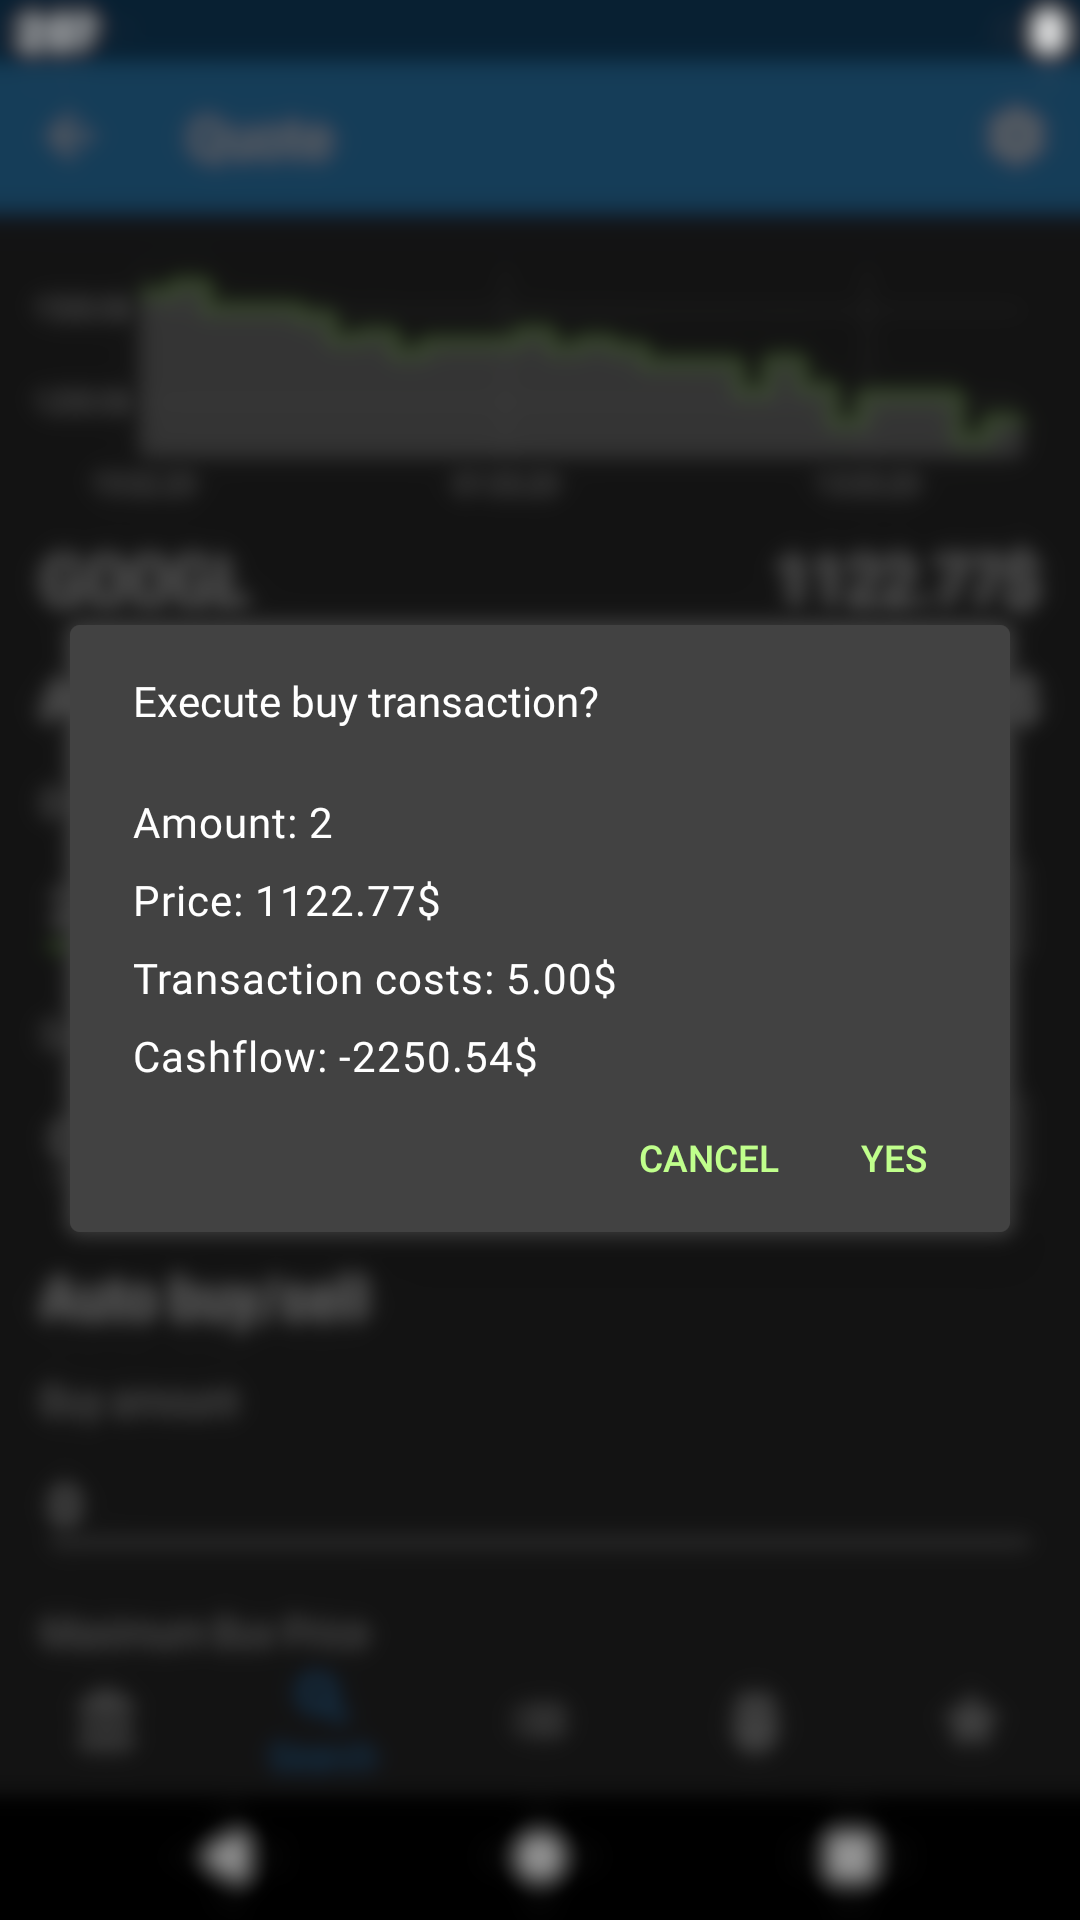
\includegraphics[height=8cm,keepaspectratio]{./images/quote/buy_dialog.png}
		\caption{Bestätigungsdialog}
		\label{fig:functionality:buy-sell:dialog}
	\end{subfigure}
	\begin{subfigure}{.5\textwidth}
		\centering
		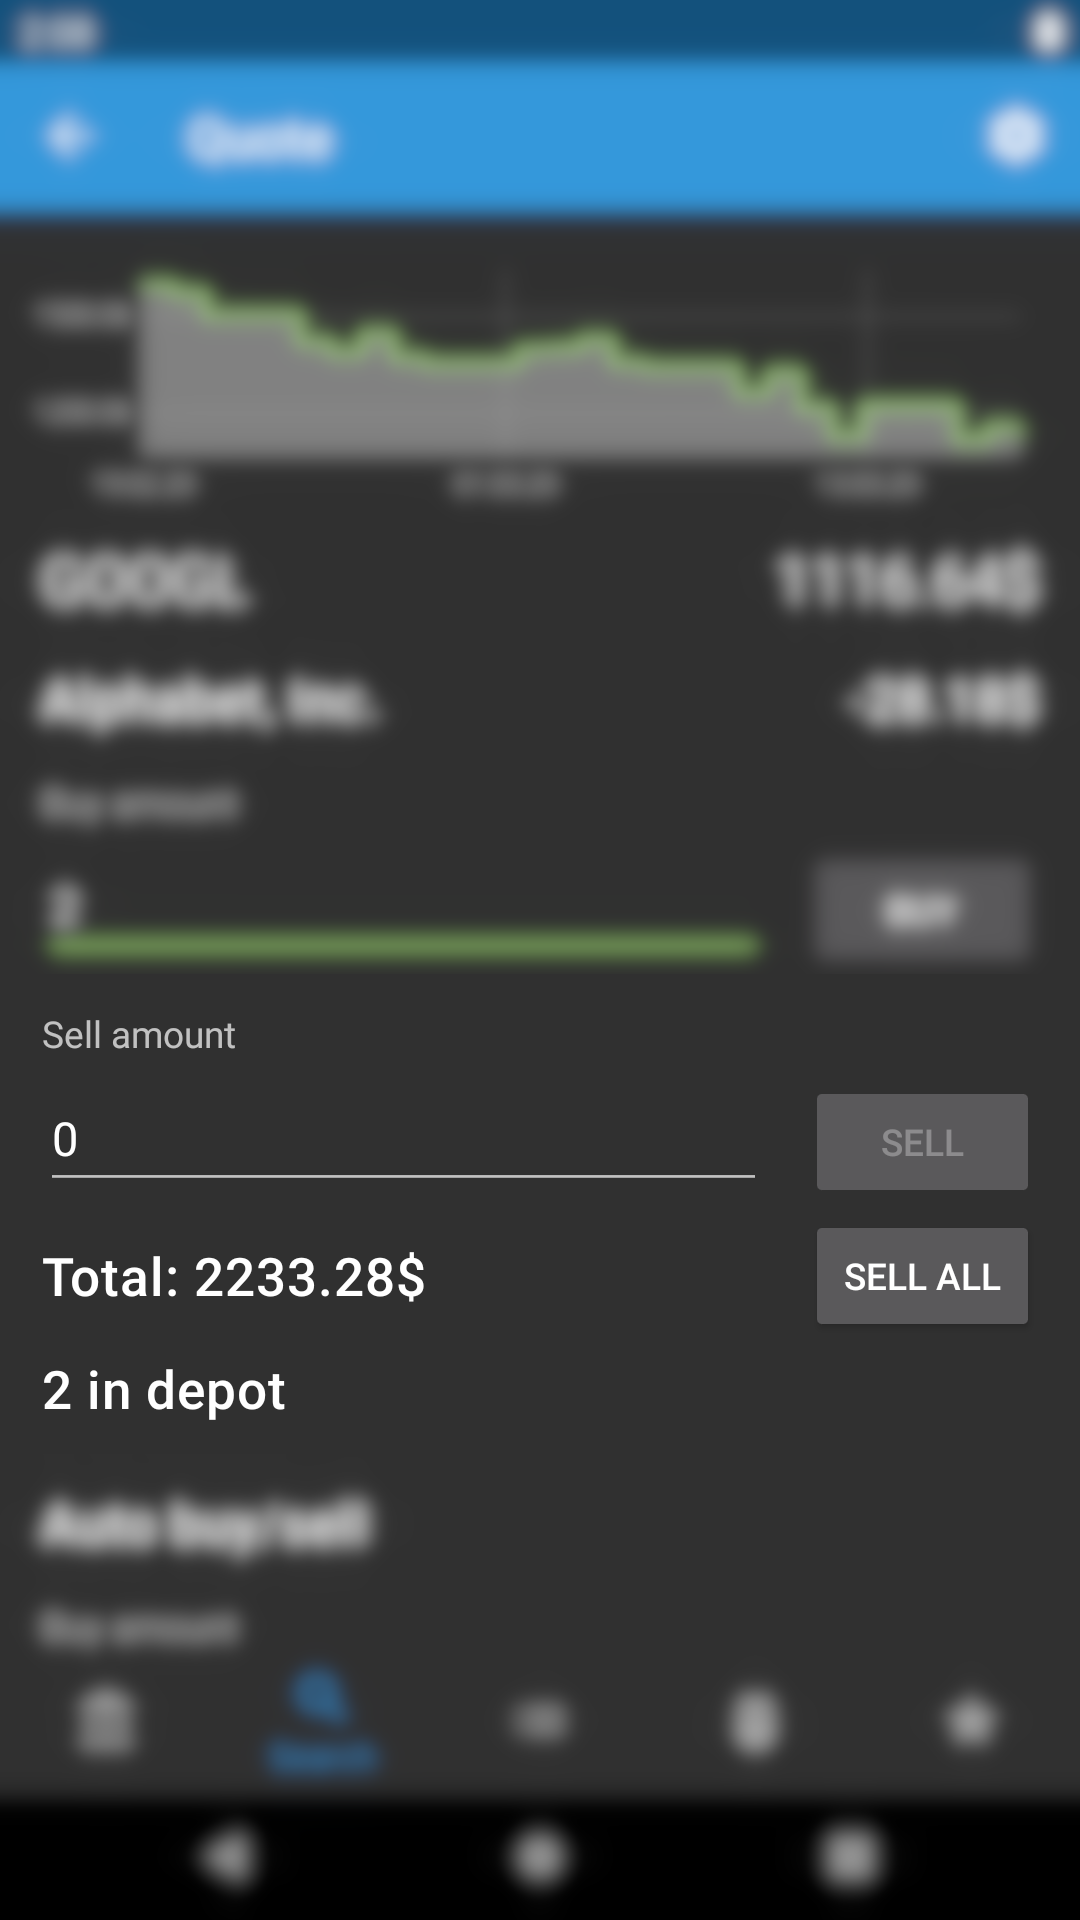
\includegraphics[height=8cm,keepaspectratio]{./images/quote/in_depot.png}
		\caption{Anlagegut im Depot}
		\label{fig:functionality:buy-sell:in-depot}
	\end{subfigure}
	\caption{Kaufen und Verkaufen}
	\label{fig:functionality:buy-sell}
\end{figure}

\autoref{fig:functionality:stockbrot:addremove} zeigt einen Abschnitt aus der Detailansicht, welcher das Hinzufügen einer Anlage zum Bot (\autoref{fig:functionality:stockbrot:add}) sowie das Entfernen dieser (\autoref{fig:functionality:stockbrot:remove}) ermöglicht. Im Abschnitt, der mit dem Label "`Auto buy/sell"' beginnt, können Kauf- und Verkaufsoptionen für den Bot festgelegt werden. Ohne Spezifikation der Kaufoptionen, wird die Anlage nicht vom Bot gekauft und ohne Spezifikation der Verkaufsoption, nicht verkauft. Wenn weder Kauf- noch Verkaufsoptionen korrekt spezifiziert wurden, bleibt der Button "`ADD TO STOCKBROT"' ausgegraut. Das Kaufverhalten des Bots kann mittels Textfeld "`Buy amount"' und "`Maximum Buy Price"' festgelegt werden. Mit diesen Optionen wird die maximale Anzahl der zu kaufenden Aktien oder Kryptowährungen, sowie der Schwellwert des Preises festgelegt, unter dem ein Kauf stattfinden soll. Mittels der Textfelder "`Minimum Sell Price"' kann festgelegt werden, welche Grenze der Preis der Anlage überschreiten muss, damit der Bot einen Verkauf durchführt. Wird eine Aktie oder Kryptowährung bereits von dem Bot kontrolliert, kann diese mittels Klick auf den Button "`REMOVE QUOTE FROM STOCKBROT"' wieder der Kontrolle des Bots entzogen werden.

\begin{figure}[H]
    \begin{subfigure}{.5\textwidth}
        \centering
        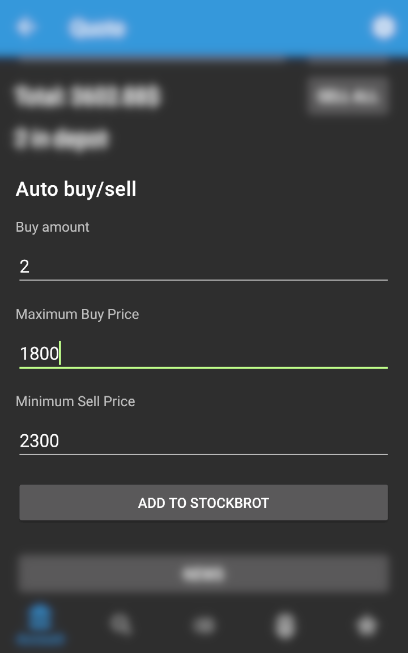
\includegraphics[height=8cm,keepaspectratio]{./images/stockbrot_add_before.png}
        \caption{Anlage zum Stockbrot hinzufügen}
        \label{fig:functionality:stockbrot:add}
    \end{subfigure}
    \begin{subfigure}{.5\textwidth}
        \centering
        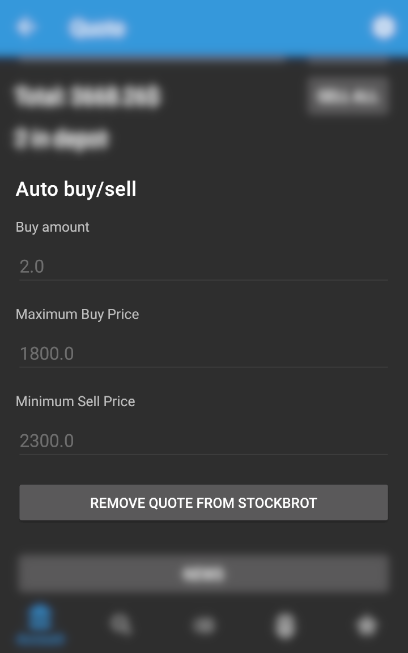
\includegraphics[height=8cm,keepaspectratio]{./images/stockbrot_add_after.png}
        \caption{Anlage vom Stockbrot entfernen}
        \label{fig:functionality:stockbrot:remove}
    \end{subfigure}
    \caption{Anlage zum/vom Stockbrot hinzufügen/entfernen}
    \label{fig:functionality:stockbrot:addremove}
\end{figure}

Im unteren Teil des Screens befindet sich ein News Button (siehe \autoref{fig:functionality:news:button}). Wenn dieser betätigt wird, werden die aktuellen Nachrichten zu der entsprechenden Anlage angezeigt. Dargestellt werden diese in einem neuen Screen, welcher in \autoref{subsec:functionality:news} beschrieben wird.

\begin{figure}[H]
    \centering
    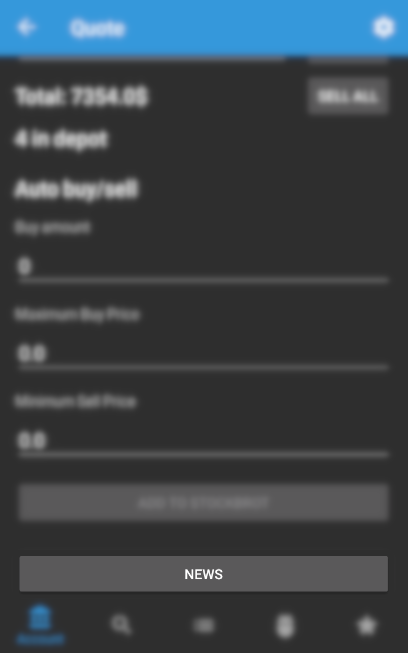
\includegraphics[height=8cm,keepaspectratio]{./images/news/news_button.png}
    \caption{News Button}
    \label{fig:functionality:news:button}
\end{figure}


\subsection{News}
\label{subsec:functionality:news}
Der News-Screen zeigt alle aktuellen Nachrichten an, die mit einer Anlage zusammenhängen (siehe \autoref{fig:functionality:news}). Dadurch, dass nur über die Detailansicht einer Anlage auf die News zugegriffen wird, wird die Anlage darüber spezifiziert. Abgerufen werden die Nachrichten über die API von IEX Cloud (siehe \autoref{subsubsec:technologies:apis:iex}). Der Screen listet, wie in \autoref{fig:functionality:news:closed} sichtbar, vorerst nur alle Nachrichtentitel auf. Falls der dazugehörige Artikel angezeigt werden soll, lässt sich jedes der Elemente durch den Pfeil auf der rechten Seite ausklappen. Anschließend wird, wie in \autoref{fig:functionality:news:open} zu sehen, zusätzlich zum Titel auch, falls vorhanden, das Bild, das Datum, die Quelle und die Beschreibung des Artikels angezeigt. Alle verfügbaren News sind in englischer Sprache verfasst.

\begin{figure}[H]
    \begin{subfigure}{.5\textwidth}
        \centering
        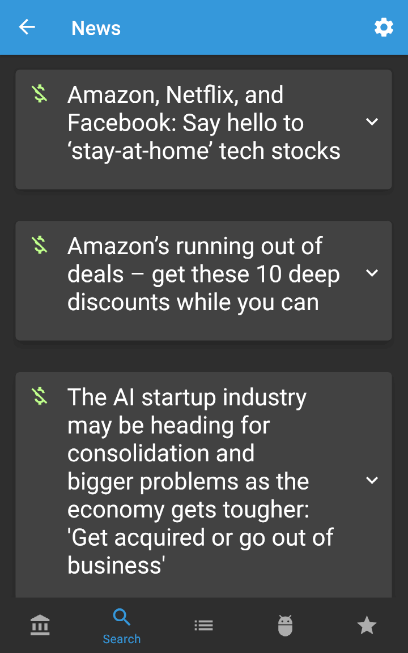
\includegraphics[height=8cm,keepaspectratio]{./images/news/news.png}
        \caption{geschlossen}
        \label{fig:functionality:news:closed}
    \end{subfigure}
    \begin{subfigure}{.5\textwidth}
        \centering
        
\includegraphics[height=8cm,keepaspectratio]{./images/news/news_open.png}
        \caption{geöffnet}
        \label{fig:functionality:news:open}
    \end{subfigure}
    \caption{News Übersicht}
    \label{fig:functionality:news}
\end{figure}


\subsection{Einstellungen}
\label{subsec:functionality:settings}
Der \textit{Settings-Screen} beinhaltet Optionen zum Zurücksetzen von Spieldaten, Aktualisieren der verfügbaren Anlagen sowie Hinzufügen und Entfernen einer Fin\-ger\-abdruck-Sperre.
Wie in \autoref{fig:functionality:settings} zu sehen sind Buttons der zuvor beschriebenen Optionen vertikal angeordnet.

\begin{figure}[H]
	\centering
	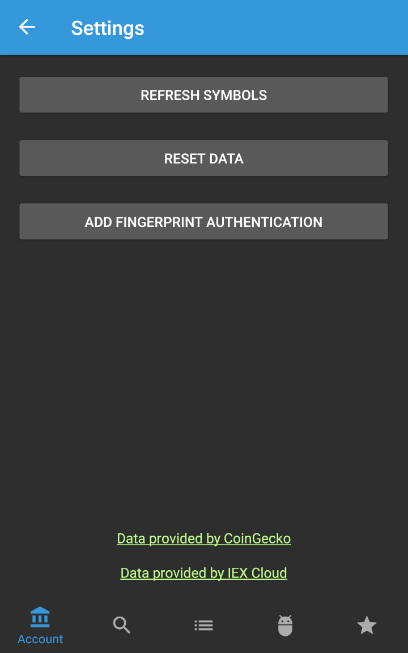
\includegraphics[width=.5\textwidth,height=8cm,keepaspectratio]{./images/settings/raw.png}
	\caption{Einstellungen}
	\label{fig:functionality:settings}
\end{figure}


Über den Button "`REFRESH SYMBOLS"' (\autoref{fig:functionality:settings:refreshsymbols:button}) ist der Benutzer in der Lage, die über die Suche verfügbaren Anlagen der CoinGecko und IEX Cloud API (siehe \autoref{subsubsec:technologies:apis:coingecko} bzw. \autoref{subsubsec:technologies:apis:iex}), zu aktualisieren. Sobald der Button geklickt wurde, wird dieser deaktiviert und es erscheint eine Benachrichtigung (\autoref{fig:functionality:settings:refreshsymbols:requested}), welche über den aktuellen Vorgang informiert. Sobald die Aktualisierung abgeschlossen ist, wird der Button wieder aktiviert und eine weitere Benachrichtigung informiert über den erfolgreichen Abschluss des Vorgangs (\autoref{fig:functionality:settings:refreshsymbols:done}).

\begin{figure}[H]
    \begin{subfigure}{.329\textwidth}
        \centering
        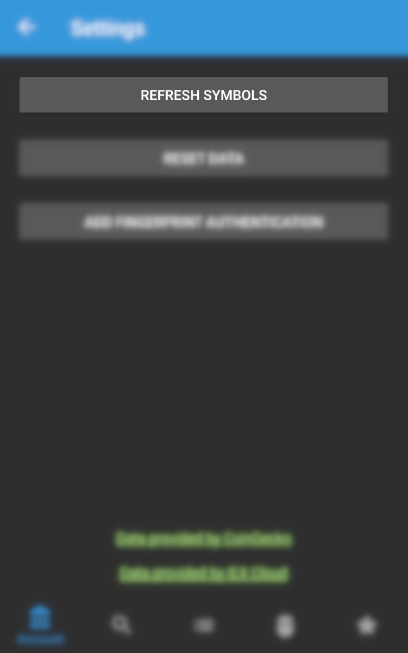
\includegraphics[height=6cm,keepaspectratio]{./images/settings/refresh_symbols_button.png}
        \caption{Button}
        \label{fig:functionality:settings:refreshsymbols:button}
    \end{subfigure}
    \begin{subfigure}{.329\textwidth}
        \centering
        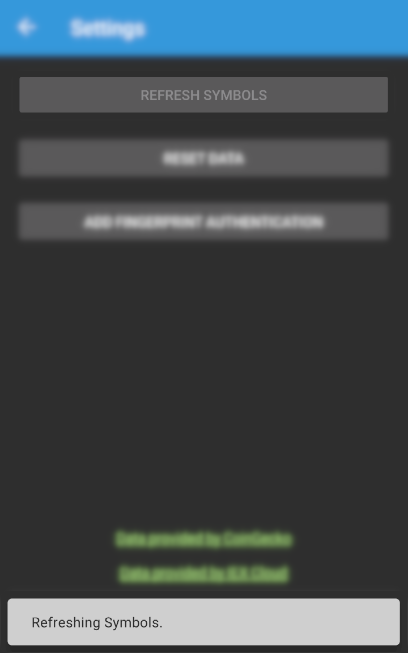
\includegraphics[height=6cm,keepaspectratio]{./images/settings/refresh_symbols_requested.png}
        \caption{Aktualisierung gestartet}
        \label{fig:functionality:settings:refreshsymbols:requested}
    \end{subfigure}
    \begin{subfigure}{.329\textwidth}
        \centering
        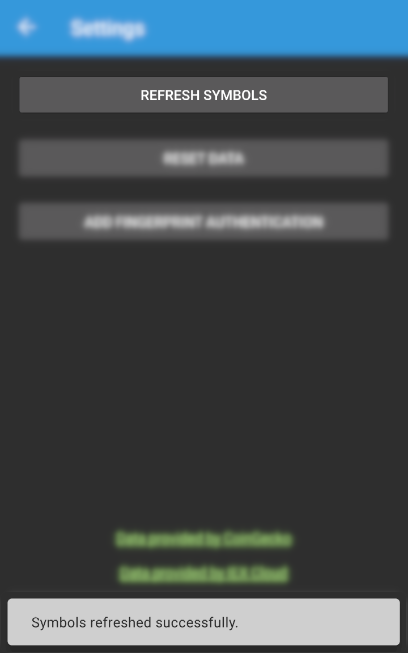
\includegraphics[height=6cm,keepaspectratio]{./images/settings/refresh_symbols_done.png}
        \caption{Aktualisierung beendet}
        \label{fig:functionality:settings:refreshsymbols:done}
    \end{subfigure}
    \caption{Symbole aktualisieren}
    \label{fig:functionality:settings:refreshsymbols}
\end{figure}


Darunter befindet sich der Button mit dem Titel "`RESET DATA"' (siehe \autoref{fig:functionality:settings:datareset:button}). Dieser ermöglicht das Zurücksetzen des Spielstands. Sobald der Button betätigt und die Daten zurückgesetzt wurden, erscheint eine Benachrichtigung (\autoref{fig:functionality:settings:datareset:notification}), welche den Abschluss des Prozesses ankündigt.

\begin{figure}[H]
    \begin{subfigure}{.5\textwidth}
        \centering
        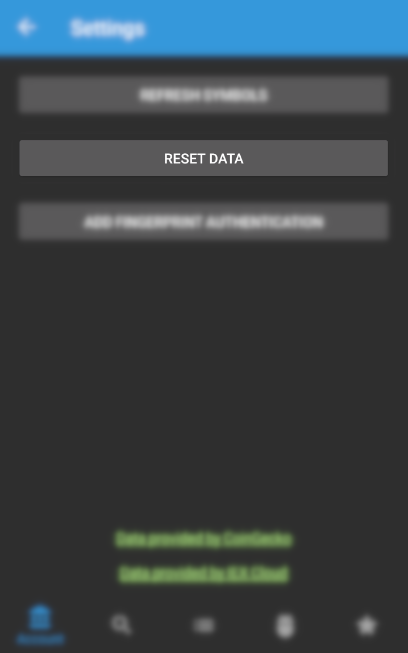
\includegraphics[height=8cm,keepaspectratio]{./images/settings/data_reset_button.png}
        \caption{Button}
        \label{fig:functionality:settings:datareset:button}
    \end{subfigure}
    \begin{subfigure}{.5\textwidth}
        \centering
        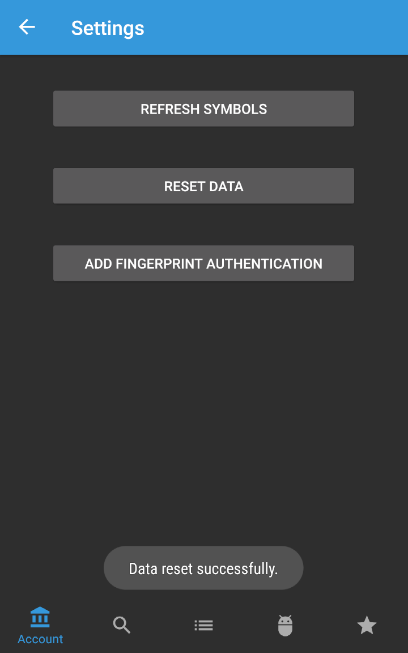
\includegraphics[height=8cm,keepaspectratio]{./images/settings/data_reset_done.png}
        \caption{Benachrichtigung}
        \label{fig:functionality:settings:datareset:notification}
    \end{subfigure}
    \caption{Daten zurücksetzen}
    \label{fig:functionality:settings:datareset}
\end{figure}


Der unterste Button "`ADD FINGERPRINT AUTHENTICATION"' ermöglicht das Schützen der Applikation durch eine Fingerabdruck-Authentifizierung (siehe \autoref{fig:functionality:settings:fingerprint:button}). Wenn diese aktiviert wurde, muss die Anwendung mit jedem Start mit dem im Android-System hinterlegten Fingerabdruck entsperrt werden. Falls kein Fingerabdruck im System hinterlegt wurde, bleibt der Button deaktiviert und ein Informationstext unter diesem Button weißt Nutzer auf den Zustand hin (siehe \autoref{fig:functionality:settings:fingerprint:notregistered}). Wenn das Hinzufügen der Fingerabdruck-Authentifizierung durch einen Klick auf den aktivierten Button gestartet wurde, erscheint ein Popup, welches den Benutzer auffordert seinen Fingerabdruck zu bestätigen (siehe \autoref{fig:functionality:settings:fingerprint:requested}). Nach der Bestätigung erscheint eine Benachrichtigung, welche den Benutzer über den Erfolgszustand informiert (siehe \autoref{fig:functionality:settings:fingerprint:done}). Wird die Bestätigung über den Button "`CANCEL"' abgebrochen, bestätigt eine Benachrichtigung den Abbruch (siehe \autoref{fig:functionality:settings:fingerprint:canceled}). Falls der Fingerabdruck nicht mit dem im System hinterlegten Abdruck übereinstimmt, wird der Benutzer darüber ebenfalls informiert (siehe \autoref{fig:functionality:settings:fingerprint:failed}).

\begin{figure}[H]
    \begin{subfigure}{.329\textwidth}
        \centering
        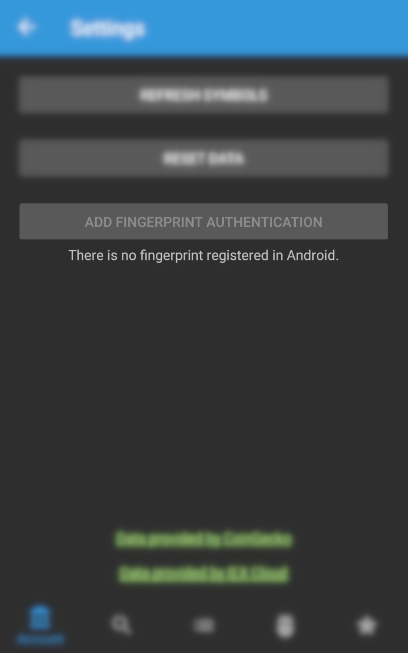
\includegraphics[height=6cm,keepaspectratio]{./images/settings/fingerprint_not_registered.png}
        \caption{Authentifizierung nicht möglich}
        \label{fig:functionality:settings:fingerprint:notregistered}
    \end{subfigure}
    \begin{subfigure}{.329\textwidth}
        \centering
        
\includegraphics[height=6cm,keepaspectratio]{./images/settings/fingerprint_button.png}
        \caption{Button\linebreak}
        \label{fig:functionality:settings:fingerprint:button}
    \end{subfigure}
    \begin{subfigure}{.329\textwidth}
        \centering
        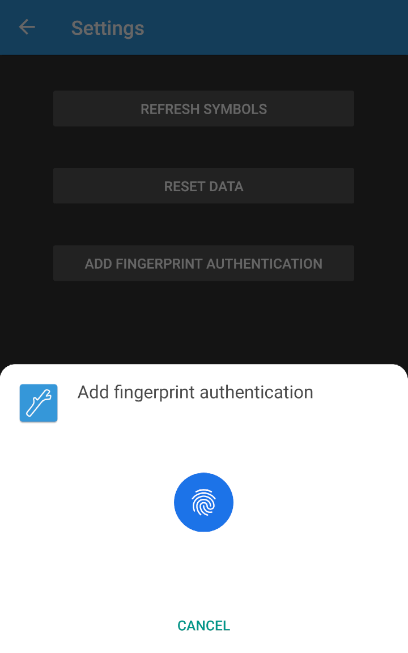
\includegraphics[height=6cm,keepaspectratio]{./images/settings/fingerprint_add_requested.png}
        \caption{Authentifizierung gestartet}
        \label{fig:functionality:settings:fingerprint:requested}
    \end{subfigure}
    \begin{subfigure}{.329\textwidth}
        \centering
        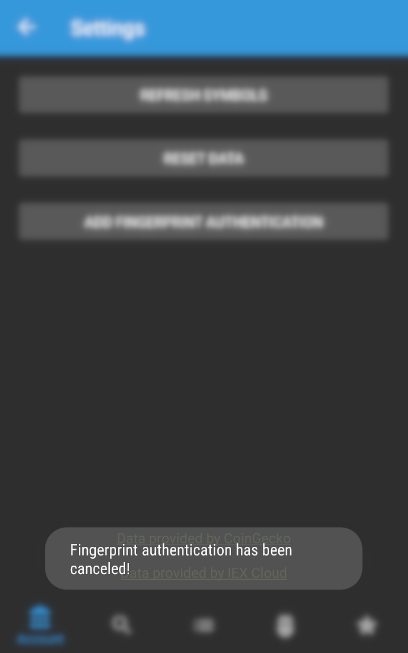
\includegraphics[height=6cm,keepaspectratio]{./images/settings/fingerprint_add_canceled.png}
        \caption{Authentifizierung abgebrochen}
        \label{fig:functionality:settings:fingerprint:canceled}
    \end{subfigure}
    \begin{subfigure}{.329\textwidth}
        \centering
        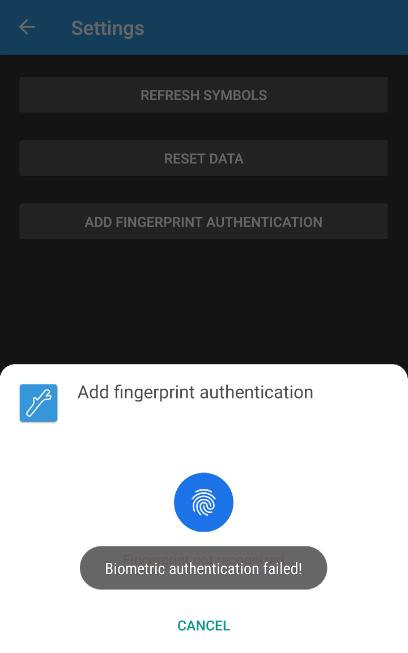
\includegraphics[height=6cm,keepaspectratio]{./images/settings/fingerprint_add_failed.png}
        \caption{Authentifizierung fehlgeschlagen}
        \label{fig:functionality:settings:fingerprint:failed}
    \end{subfigure}
    \begin{subfigure}{.329\textwidth}
        \centering
        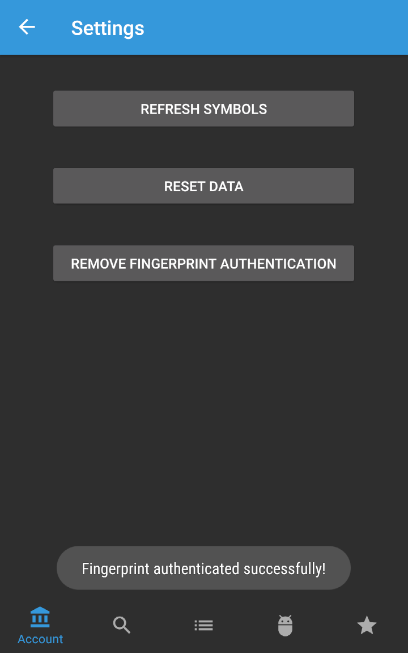
\includegraphics[height=6cm,keepaspectratio]{./images/settings/fingerprint_add_done.png}
        \caption{Authentifizierung abgeschlossen}
        \label{fig:functionality:settings:fingerprint:done}
    \end{subfigure}
    \caption{Fingerabdruck-Authentifizierung}
    \label{fig:functionality:settings:fingerprint}
\end{figure}


Am unteren Ende des Screens (siehe \autoref{fig:functionality:settings:attributions}) befinden sich die notwendigen Zuschreibungen an die verwendeten Schnittstellen (siehe \autoref{subsec:technologies:apis}).
Durch Klicken auf einen der Links werden Nutzer zur Website der jeweiligen Schnittstelle weitergeleitet.

\begin{figure}[H]
    \centering
    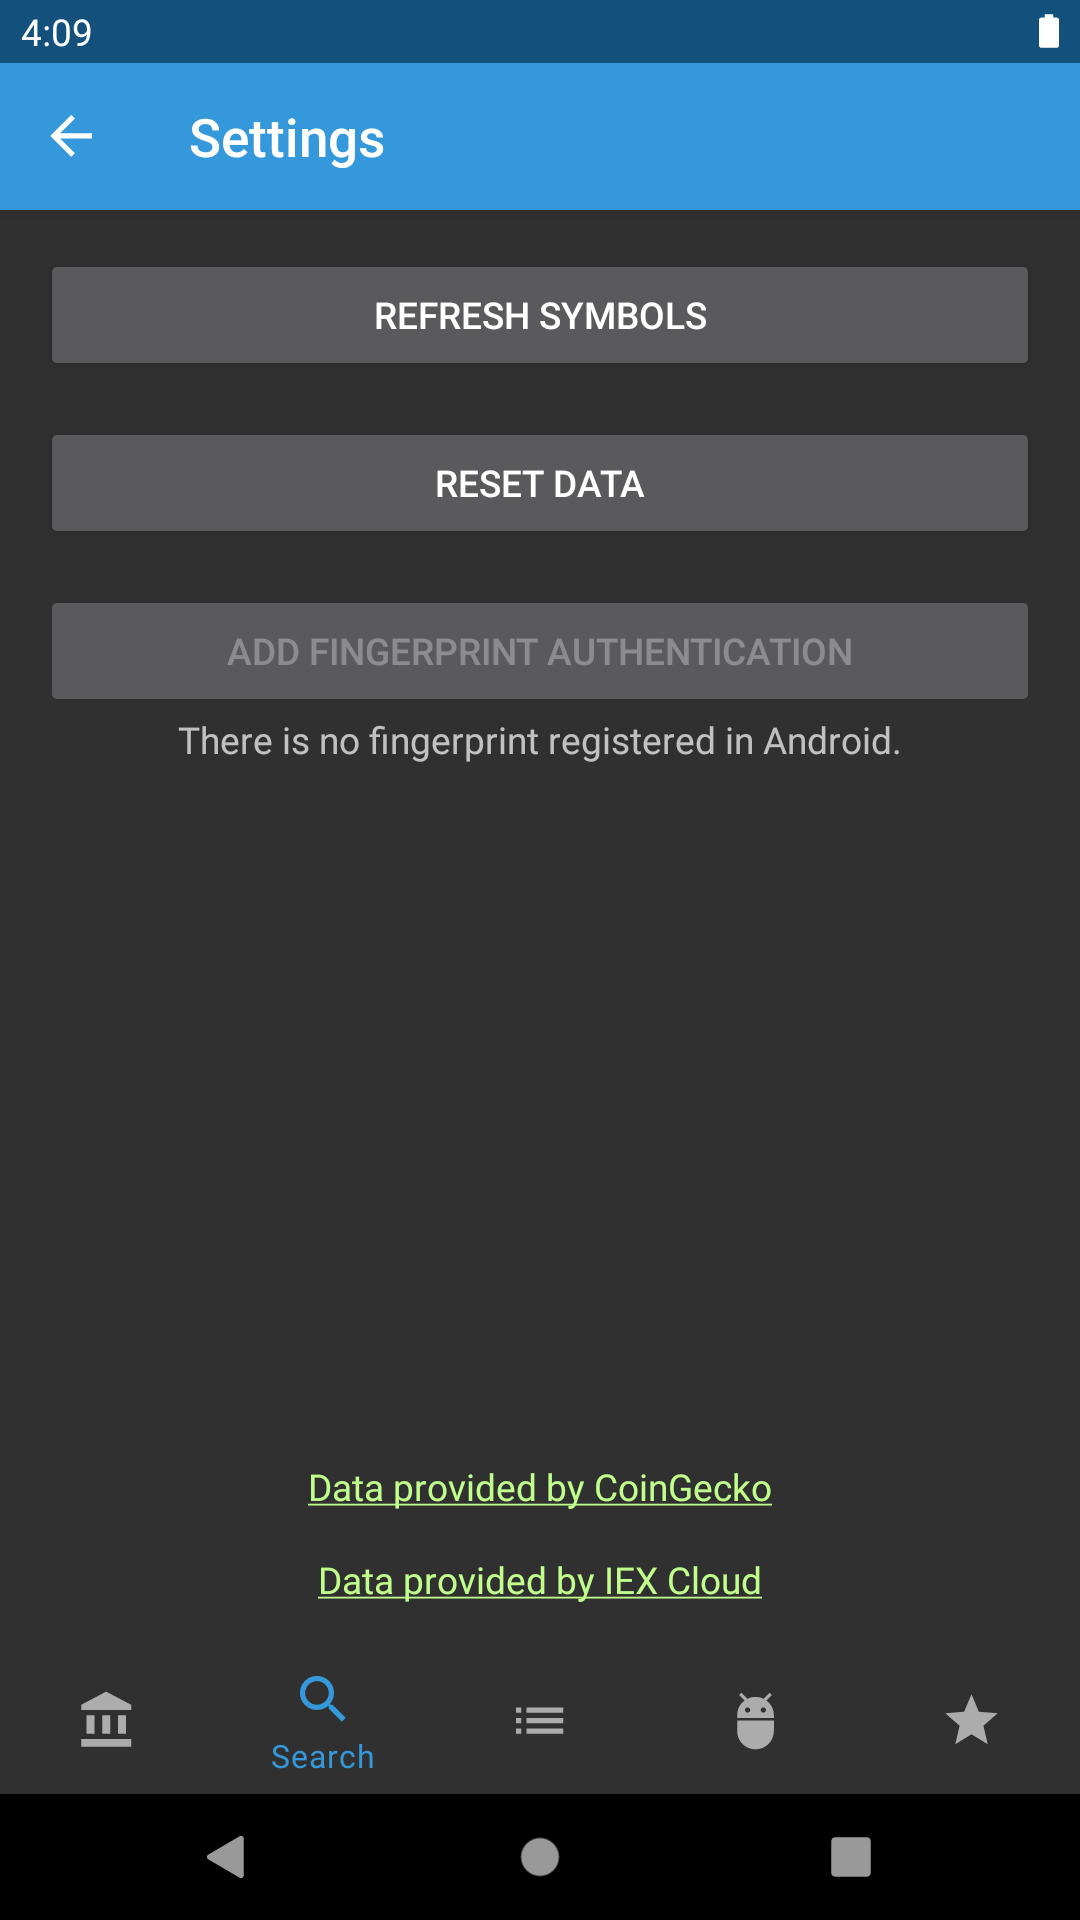
\includegraphics[width=.5\textwidth,height=8cm,keepaspectratio]{./images/settings/attribution.png}
    \caption{Zuschreibungen}
    \label{fig:functionality:settings:attributions}
\end{figure}

\section{Demonstration}
\label{sec:demo}
Um die Funktionen und die Handhabung der Applikation zu demonstrieren, werden im Folgenden einige typische Anwendungsfälle und Transaktionen durchgespielt. Nach dem Start der Applikation wird dem Nutzer der Account-Bildschirm angezeigt. Wie in \autoref{fig:demo:start} zu sehen, verfügt der Nutzer zu Beginn über einen Kontostand von 10.000,- \$ und kein Anlagevermögen (0,00 \$), d. h. ein leeres (Wertpapier-) Depot. Die Wertentwicklung seines Gesamtvermögens, in der App als \textit{Performance} ausgewiesen, beträgt zu Beginn des Spiels ebenfalls 0.00 \%.

\begin{figure}[H]
	\centering
	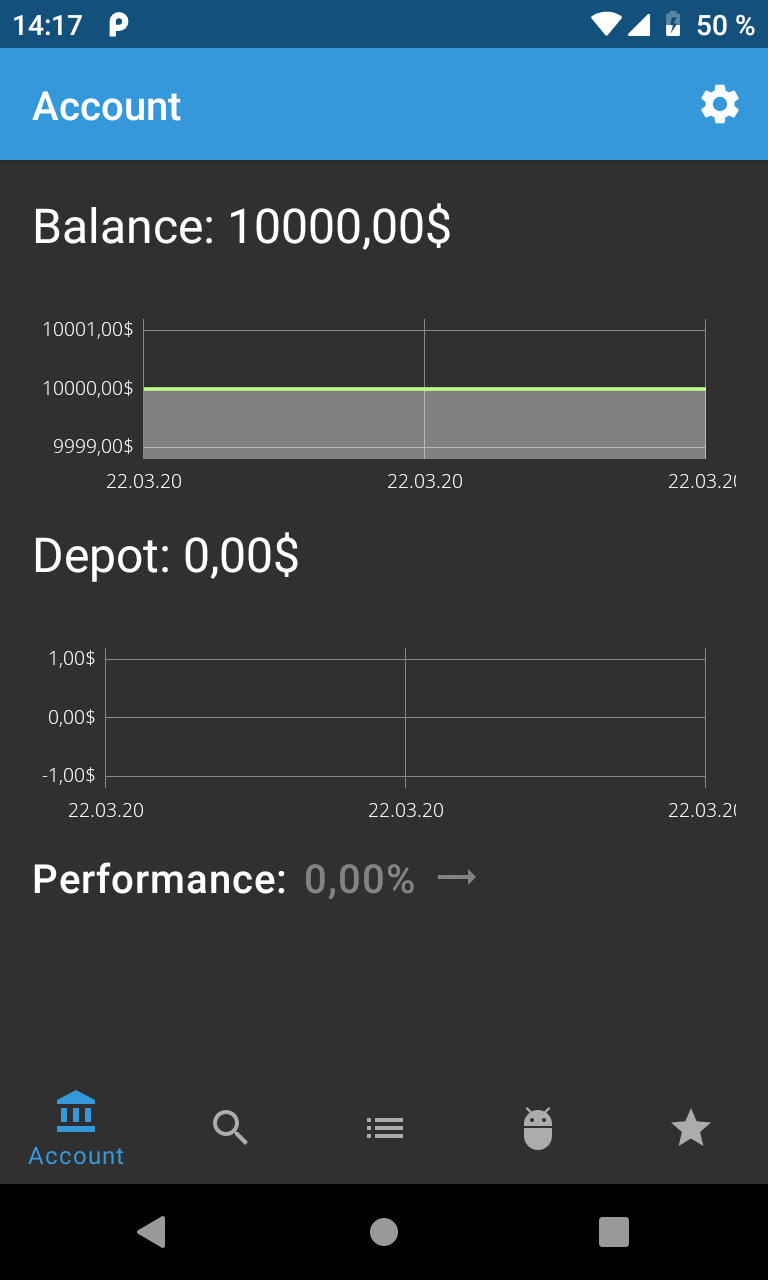
\includegraphics[width=.5\textwidth,height=8cm,keepaspectratio]{./images/demo/start.png}
	\caption{Account}
	\label{fig:demo:start}
\end{figure}

 Um von den steigenden Aktienkursen zu profitieren, wollen wir uns eine Aktie des Unternehmens Agilent Technologies\footnote{Ein amerikanisches Technologieunternehmen mit Sitz in Santa Clara, Kalifornien, das analytische Messgeräte herstellt.} kaufen. Dazu klicken wir in der Bottom-Navigation den Search-Button und wechseln zum Search-Bildschirm.

\begin{figure}[H]
	\begin{subfigure}{.5\textwidth}
		\centering
		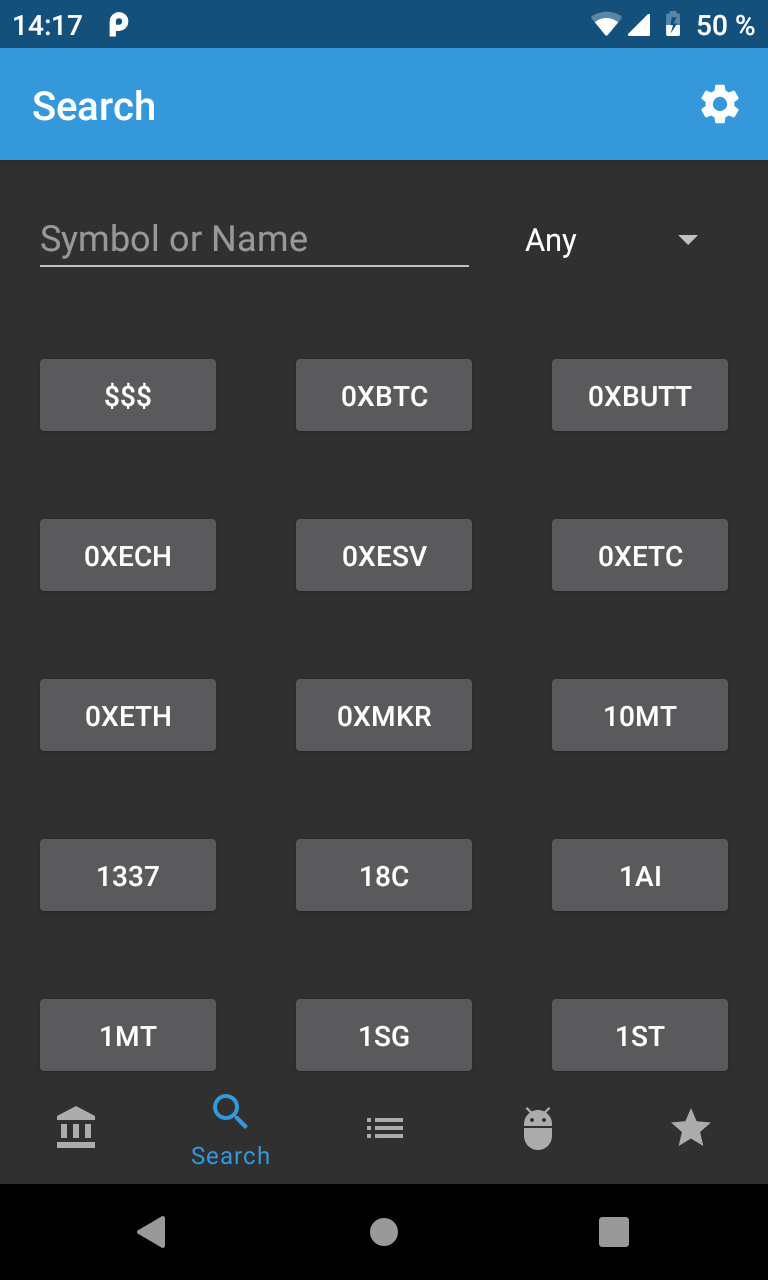
\includegraphics[height=8cm,keepaspectratio]{./images/demo/search.png}
		\caption{Search-Bildschirm}
		\label{fig:demo:search_screen}
	\end{subfigure}
	\begin{subfigure}{.5\textwidth}
		\centering
		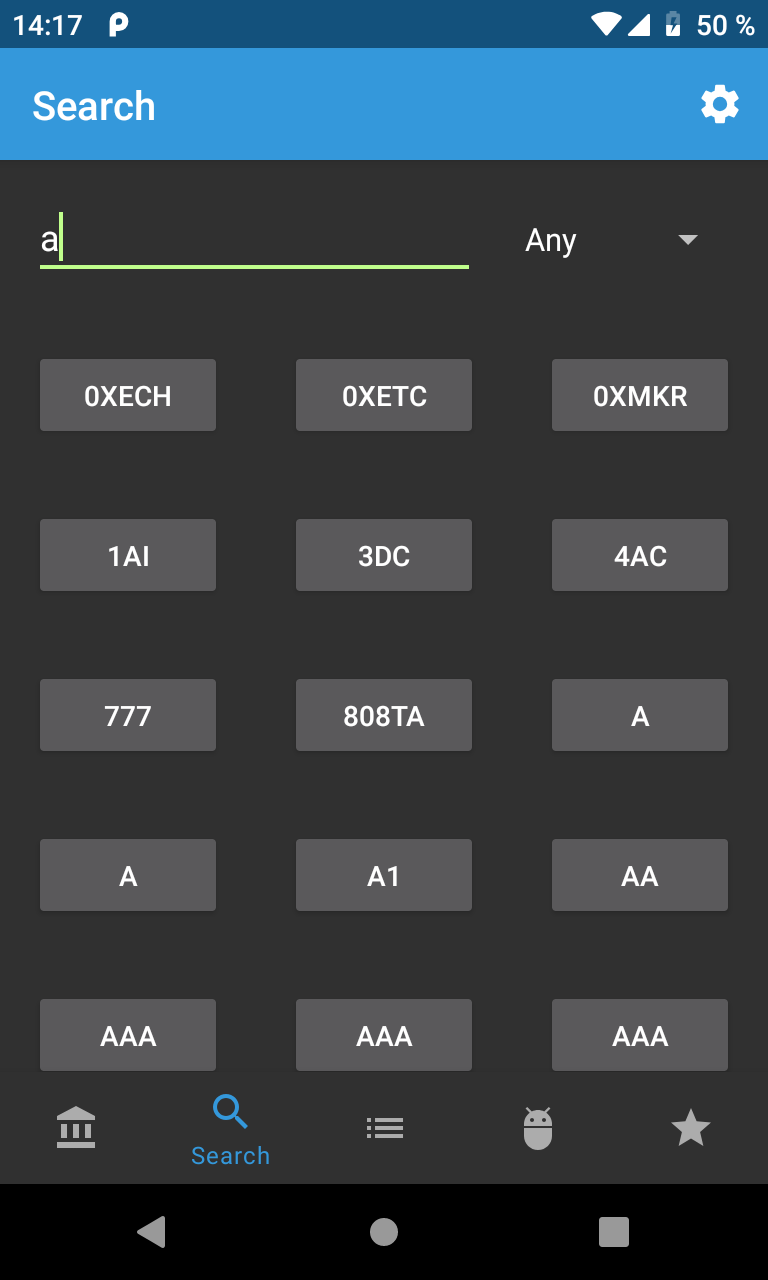
\includegraphics[height=8cm,keepaspectratio]{./images/demo/search_a.png}
		\caption{Suche - Filter nach "`a"'}
		\label{fig:demo:search_a}
	\end{subfigure}
	\caption{Suche}
	\label{fig:demo:search}
\end{figure}

\autoref{fig:demo:search_screen} zeigt den Search-Bildschirm. In diesem werden, nach einer kurzen Aktualisierung, zunächst alle Anlagemöglichkeiten, d. h. Aktien und Kryptowährungen, in alphabetischer Reihenfolge angezeigt. Um die gewünschte Aktie zu finden, geben wir in das Suchfeld den Buchstaben "`a"' ein. Hierauf werden alle Anlagemöglichkeiten gefiltert und nur diejenigen angezeigt, deren Symbol (Abkürzung) mit "`A"' oder "`a"' beginnt oder deren Namen eine "`A"' bzw. "`a"' enthalten. Dies wird in \autoref{fig:demo:search_a} dargestellt. Wir wählen die erste Wertanlage, die durch "`A"' dargestellt ist, aus und gelangen zum Quote-Bildschirm. Dieser bietet eine Detailansicht über die ausgewählte Aktie und ist in \autoref{fig:demo:quote} zu sehen. Hier werden uns die Wertentwicklung der Aktie im letzten Monat in Form eines Diagramms, der aktuelle Wert der Aktie sowie die Veränderung des Kurses gegenüber dem Vortag angezeigt.

\begin{figure}[H]
	\centering
	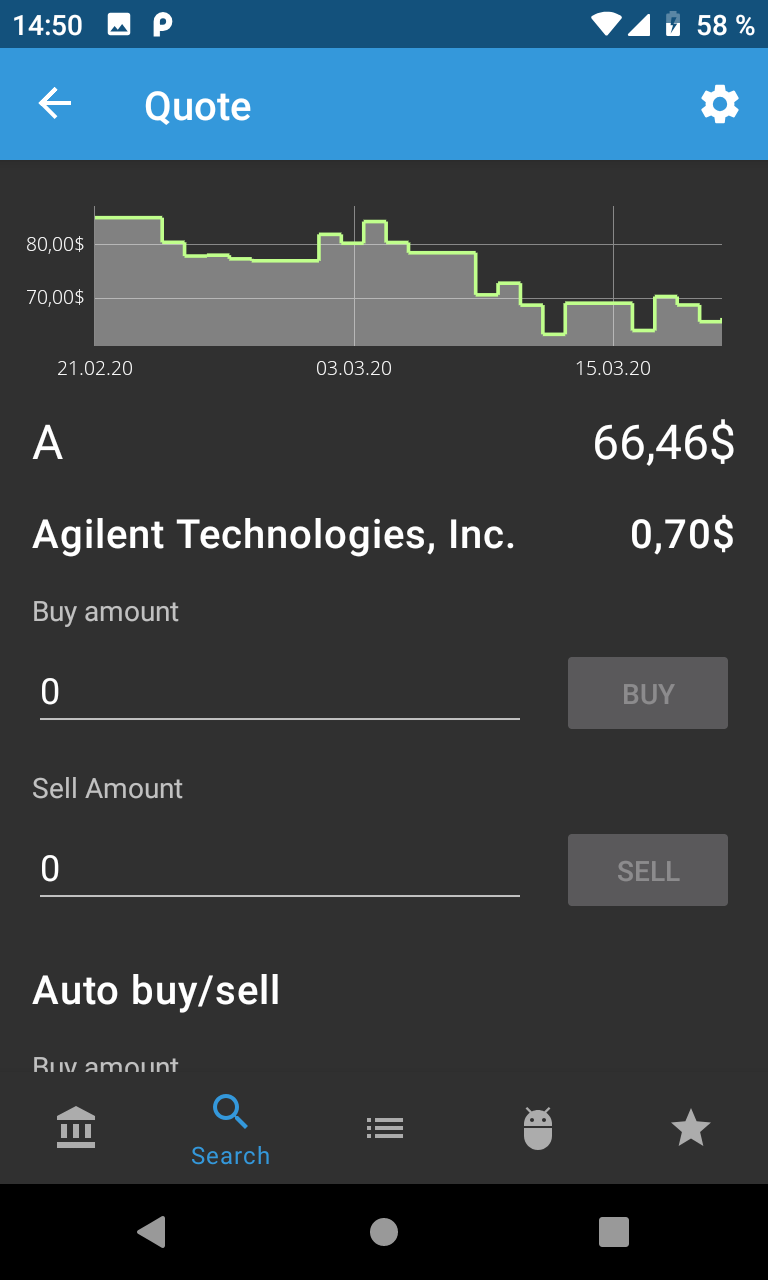
\includegraphics[height=8cm,keepaspectratio]{./images/demo/quote.png}
	\caption{Quote}
	\label{fig:demo:quote}
\end{figure}

Um Aktien dieses Unternehmens zu erwerben, geben wir eine Kaufmenge von 12 in das vorgesehene Eingabefeld ein, wie in \autoref{fig:demo:buy_a} dargestellt. Nach Betätigen des BUY-Buttons erscheint ein Dialog, der die Transaktion zusammenfasst und uns auffordert den Kauf zu bestätigen. Dies ist in \autoref{fig:demo:buy_a_confirm} zu sehen.

\begin{figure}[H]
	\begin{subfigure}{.5\textwidth}
		\centering
		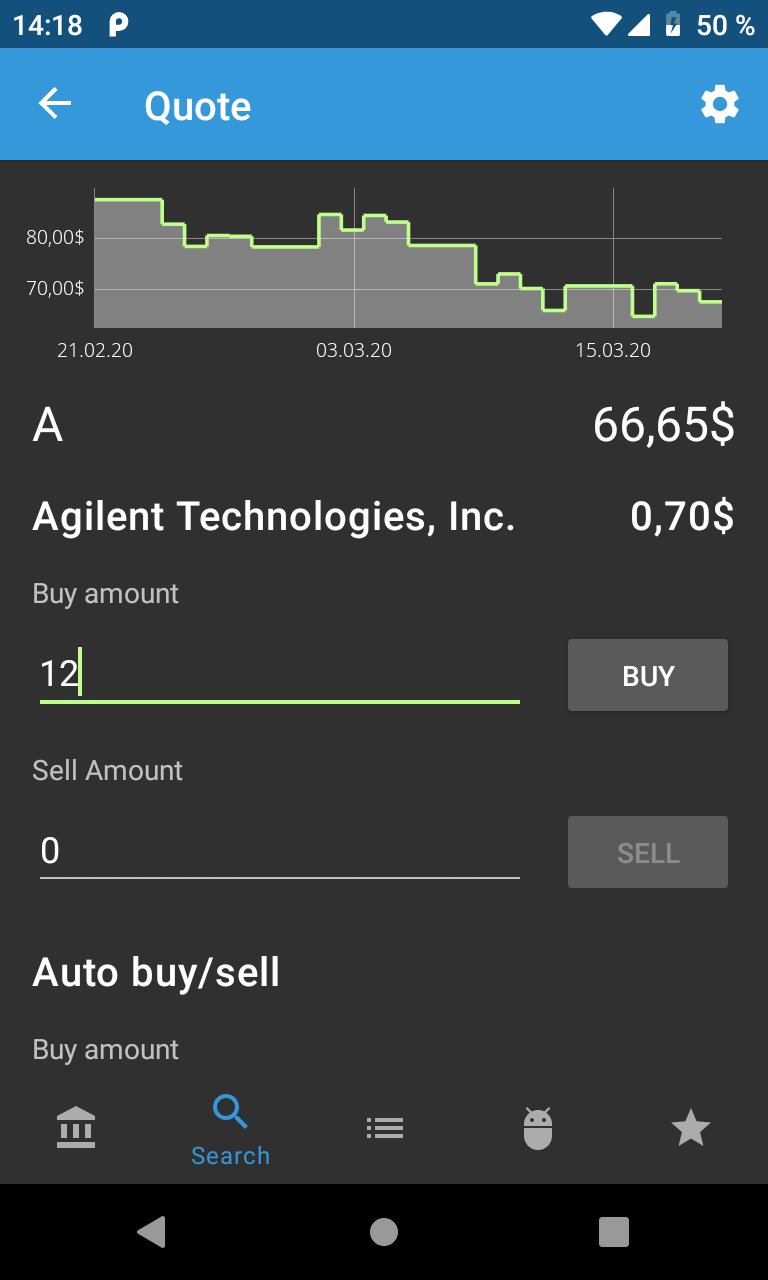
\includegraphics[height=8cm,keepaspectratio]{./images/demo/buy_a.png}
		\caption{Kauf von 12 Aktien}
		\label{fig:demo:buy_a}
	\end{subfigure}
	\begin{subfigure}{.5\textwidth}
		\centering
		\includegraphics[height=8cm,keepaspectratio]{./images/demo/buy_a_confirm.png}
		\caption{Kaufbestätigung}
		\label{fig:demo:buy_a_confirm}
	\end{subfigure}
	\caption{Kauf}
	\label{fig:demo:buy}
\end{figure}

Da wir nicht jeden Aktienkauf und -verkauf persönlich durchführen möchten, fügen wir diese Aktie dem automatischen Handel durch den Bot (stockbrot) hinzu. 

\begin{figure}[H]
	\begin{subfigure}{.5\textwidth}
		\centering
		\includegraphics[height=8cm,keepaspectratio]{./images/demo/add_stockbot.png}
		\caption{Automatischer Handel}
		\label{fig:demo:add_stockbot}
	\end{subfigure}
	\begin{subfigure}{.5\textwidth}
		\centering
		\includegraphics[height=8cm,keepaspectratio]{./images/demo/added_stockbot_view.png}
		\caption{Automatisch gehandelte Anlagen}
		\label{fig:demo:added}
	\end{subfigure}
	\caption{Stockbrot}
	\label{fig:demo:bot}
\end{figure}

Hierzu geben wir 60,00 \$ als Höchstkaufpreis an. Bis zu diesem Kaufpreis soll diese Aktie automatisch gekauft werden. Als Verkaufspreis geben wir 70,00 \$ an. Ab diesem Wert wird die Aktie automatisch für uns verkauft, so wie in \autoref{fig:demo:add_stockbot} zu sehen. Einen Überblick über alle automatisch gehandelten Anlagen bietet der Stockbrot-Bildschirm, den wir über die Bottom-Navigation erreichen. Hier sind die Kauf- und Verkaufspreise für den automatischen Handel nochmals aufgeführt, zu sehen in  \autoref{fig:demo:added}.\newline
Des Weiteren können wir uns im Quote-Bildschirm aktuelle Nachrichten zum Aktienwert und dem jeweiligen Unternehmen anzeigen lassen. Diese sehen wir in \autoref{fig:demo:news}.

\begin{figure}[H]
	\centering
	\includegraphics[height=8cm,keepaspectratio]{./images/demo/news.png}
	\caption{Nachrichten}
	\label{fig:demo:news}
\end{figure}

Als nächstes wollen wir drei der erworbenen Aktien manuell wieder verkaufen, um über mehr ungebundenes Kapital zu verfügen. Hierfür geben wir im Quote-Bildschirm die Zahl "`3"' im dafür vorgesehenen Eingabefeld ein, siehe \autoref{fig:demo:sell_a_three}. Erneut müssen wir die Transaktion bestätigen, wie in \autoref{fig:demo:sell_a_confirmation} zu sehen ist.

\begin{figure}[H]
	\begin{subfigure}{.5\textwidth}
		\centering
		\includegraphics[height=8cm,keepaspectratio]{./images/demo/sell.png}
		\caption{Verkauf von drei Aktien}
		\label{fig:demo:sell_a_three}
	\end{subfigure}
	\begin{subfigure}{.5\textwidth}
		\centering
		\includegraphics[height=8cm,keepaspectratio]{./images/demo/sell_a_confirmation.png}
		\caption{Verkaufsbestätigung}
		\label{fig:demo:sell_a_confirmation}
	\end{subfigure}
	\caption{Verkauf}
	\label{fig:demo:sell_a}
\end{figure}

Einen Überblick über alle bisherigen Transaktionen erhalten wir im History-Bildschirm, den wir über die Bottom-Navigation erreichen. 

\begin{figure}[H]
	\begin{subfigure}{.5\textwidth}
		\centering
		\includegraphics[height=8cm,keepaspectratio]{./images/demo/history_closed.png}
		\caption{Bisheriger Kauf und Verkauf}
		\label{fig:demo:history_closed}
	\end{subfigure}
	\begin{subfigure}{.5\textwidth}
		\centering
		\includegraphics[height=8cm,keepaspectratio]{./images/demo/history_open.png}
		\caption{ Detailansicht}
		\label{fig:demo:history_open}
	\end{subfigure}
	\caption{Transaktionshistorie}
	\label{fig:demo:history}
\end{figure}

Wie in \autoref{fig:demo:history_closed} zu sehen, werden unser Kauf und Verkauf in Form von ausklappbaren Karten dargestellt. Das Verkaufssymbol (Dollar) zeichnet einen Verkauf aus und das Kaufsymbol (Einkaufswagen) weist Anlagekäufe aus. Nachdem wir beide Karten öffnen, können wir uns die Details dieser Transaktionen anschauen, siehe \autoref{fig:demo:history_open}. Bei Verkäufen wird zusätzlich die Gewinn- bzw. Verlusthöhe durch diesen Verkauf aufgeführt.\newline
Durch die bisherigen Aktiengeschäfte haben wir bereits einige Errungenschaften im Spiel erreicht. Um diese zu betrachten, wechseln wir über die Bottom-Navigation zum Achievements-Bildschirm, wie in \autoref{fig:demo:achievements_closed} zu sehen. So haben wir bereits die Errungenschaften "`Eine Aktie im Depot"', "`Zwei Aktien im Depot"' und "`Zehn Aktien im Depot"' freigespielt. Durch Öffnen der einzelnen Karten wird eine Beschreibung der jeweiligen Errungenschaft angezeigt, wie in  \autoref{fig:demo:achievements_open} zu sehen ist.

\begin{figure}[H]
	\begin{subfigure}{.5\textwidth}
		\centering
		\includegraphics[height=8cm,keepaspectratio]{./images/demo/achievements_closed.png}
		\caption{Erreichte Errungenschaften}
		\label{fig:demo:achievements_closed}
	\end{subfigure}
	\begin{subfigure}{.5\textwidth}
		\centering
		\includegraphics[height=8cm,keepaspectratio]{./images/demo/achievements_open.png}
		\caption{Detailansicht}
		\label{fig:demo:achievements_open}
	\end{subfigure}
	\caption{Errungenschaften}
	\label{fig:demo:achievements}
\end{figure}

\begin{figure}[H]
	\centering
	\includegraphics[height=8cm,keepaspectratio]{./images/demo/end.png}
	\caption{Account nach Kauf und Verkauf von Aktien}
	\label{fig:demo:end}
\end{figure}

Um das Ergebnis unserer Aktiengeschäfte zu ermitteln, wechseln wir über die Bottom-Navigation erneut zum Account-Bildschirm. Darin wird der aktuelle Kontostand von 9.396,48 \$ und der Wert unseres Depots in Höhe von 616,95\,\$ angezeigt. Die Wertentwicklung unseres Gesamtvermögens beträgt +0,13 \%. Unser Aktiendepot besteht aus neun Aktien der Firma Agilent Technologies.\newline
Zuletzt wollen wir unseren bisherigen Spielfortschritt löschen, indem wir alle Spieldaten zurücksetzen. Dazu wechseln wir in den Settings-Bildschirm über den dazugehörigen Button in der Kopfzeile. Darin können wir alle Informationen über die verfügbaren Anlagemöglichkeiten aktualisieren, die bisher gespeicherten Spieldaten zurückzusetzen und eine Fingerabdruckauthentifizierung aktivieren, falls ein Fingerabdrucksensor verfügbar ist, wie in \autoref{fig:demo:settings_data_reset} zu sehen ist. Nachdem wir den Reset Data-Button betätigt haben, wird uns eine Bestätigung der erfolgreichen Zurücksetzung aller Daten angezeigt, siehe \autoref{fig:demo:settings_data_reset_confirmation}.

\begin{figure}[H]
	\begin{subfigure}{.5\textwidth}
		\centering
		\includegraphics[height=8cm,keepaspectratio]{./images/demo/settings.png}
		\caption{Spieldaten zurücksetzen}
		\label{fig:demo:settings_data_reset}
	\end{subfigure}
	\begin{subfigure}{.5\textwidth}
		\centering
		\includegraphics[height=8cm,keepaspectratio]{./images/demo/settings_data_reset.png}
		\caption{Bestätigung des Zurücksetzens}
		\label{fig:demo:settings_data_reset_confirmation}
	\end{subfigure}
		\caption{Einstellungen}
		\label{fig:demo:settings}
\end{figure}


\section{Teamwork}
\label{sec:teamwork}
Eine Startschwierigkeit während der Zusammenarbeit war, dass die Entwickler im Team nicht über ähnlich gute Kenntnisse der Android-Architektur und Kotlin-Syntax verfügten. Dieses Problem wurde zum einen dadurch bewältigt, dass sich erfahrenere Entwickler mit den weniger erfahrenen austauschten und zu Beginn Pair-Programming \footnote{Siehe \url{https://en.wikipedia.org/wiki/Pair_programming}} betrieben. Durch die räumlich nahe Zusammenarbeit und ein hohes Maß an Teamfähigkeit bei allen Teammitgliedern, konnten Probleme von Einzelnen meist schnell in der Gruppe gelöst werden. Nachdem zu Beginn Aufgaben nach technischen Schichten (Layern), wie APIs und Datenbanken vergeben wurden, gingen wir schnell dazu über, die Aufgaben nach Funktionalitäten, wie Suche, Historie, Stockbrot usw. zu vergeben. Diese Aufgabenverteilung kapselte einzelne Aufgaben wesentlich besser als die vorherige nach Schichten orientierte Aufteilung. Wir verständigten uns darauf, im Sinne der agilen Softwareentwicklung in kleinschrittigem Vorgehen Erweiterungen an einem bereits in der Frühphase funktionierenden Produkt vorzunehmen. Nach kurzer Absprache verständigten wir uns darauf, unser Projekt entsprechend dem Git-Workflow Design (Gitflow) \footnote{Siehe \url{https://www.atlassian.com/git/tutorials/comparing-workflows/gitflow-workflow}} zu versionieren. Demnach verfügte unser Projekt über zwei Haupt-Branches um den Verlauf des Projekts aufzuzeichnen. Der \textit{main}-Branch enthält die offiziellen Release-Versionen des Projekts und der \textit{develop}-Branch dient dazu, die einzelnen Features zu integrieren, sobald sie fertig gestellt sind. \newline
Im Verlauf der Arbeit kristallisierten sich rasch Rollen heraus. Der erfahrenste Entwickler wurde schnell zum technischen Leiter und Ansprechpartner bei ernsteren Problemen. Ein anderes Teammitglied ging auf den Kunden (die Aufgabenstellenden) zu, um bei Unklarheiten die Aufgabenstellung zu präzisieren. Dies hat zu einem guten Arbeitsklima beigetragen. \newline
Unser Team hatte in der ganzen Woche ein positives Arbeitsklima. Jedes Teammitglied engagierte sich für das gemeinsame Ziel und trug durch kreative Ideen dazu bei, unser Projekt zu verbessern.


\section{Zusammenfassung}
\label{sec:summary}
Im Rahmen der Blockveranstaltung \textit{Code-Camp Context-Awareness 1} entwickelte unser Team ein Börsenhandelssimulationsspiel für Android. Mit dieser Applikationen können Informationen über Aktien und Kryptowährungen abgerufen werden sowie Anlagen erworben und veräußert werden. Hierbei ermöglichen Übersichten über das bestehende Depot, den Kontostand und alle bisherigen Transaktionen, das Spielgeschehen nachzuvollziehen. Der Handel kann durch einen Bot automatisiert werden. \newline
Bereits im Verlauf der Woche konnten wir alle gestellten Mindestanforderungen an unsere Börsenhandelssimulation erfüllen und darüber hinaus zahlreiche zusätzliche Funktionalitäten umsetzen.


\section{Fazit}
\label{sec:conclusion}
Für die meisten Entwickler unseres Teams war dies das erste Android-Software-Projekt, wodurch die "`Lernkurve"' zu Beginn recht steil verlief. Durch unsere gute Zusammenarbeit und unseren Einsatz für das Projekt konnten wir diese Veranstaltung dazu nutzen, neue Kenntnisse der Android-Entwicklung zu erwerben und zu vertiefen. Insgesamt waren alle Teammitglieder vom Android-"`Ökosystem"' positiv überrascht. Wir fühlen uns gut für zukünftige Android-App-Entwicklung gerüstet.


\section{Ausblick}
\label{sec:outlook}
% was kann man noch machen, was habt ihr nicht geschafft,..
Aus verschiedenen Gründen konnte das Team einige geplante Zusatzfunktionalitäten nicht umsetzen.
Dazu zählen ein Aktienhebel, auswählbare Schwierigkeitsgrade und eine Überarbeitung eines Datenbankschemas.
Die ersten beiden Funktionalitäten wurden aus Zeitmangel nicht implementiert.
Das Datenbankschema wurde zwar überarbeitet, jedoch konnte die neue Version nicht integriert werden.
Dafür verantwortlich ist ein Fehler in der verwendeten \textit{Room}-Bibliothek (siehe \autoref{subsubsec:technologies:bibs:room}), welcher zur Zeit der Entwicklung nicht behoben werden konnte.

\begingroup
\raggedright
\printbibliography[title={Referenzen}]
\endgroup


\end{document}
